\documentclass[12pt,a4paper]{article}

% ---------------------------------------------------------------------------
% PREÁMBULO
% ---------------------------------------------------------------------------
\usepackage[utf8]{inputenc}
\usepackage[T1]{fontenc}
\usepackage{lmodern}

% Español cauteloso: sin shorthands activas (evita redefiniciones de "-.,")
\usepackage[spanish,es-noshorthands]{babel}

\usepackage[a4paper, margin=2.3cm, top=2.2cm, bottom=2.2cm]{geometry}
\usepackage{pdflscape} % Permite paginas apaisadas individuales sin romper la geometria global

\usepackage{microtype}
\usepackage{setspace}
\setstretch{1.18}
\setlength{\parindent}{0pt}
\setlength{\parskip}{4pt}
\setlength{\emergencystretch}{1.5em}
\raggedbottom

\usepackage{textcomp}
\usepackage{enumitem}
\setlist{leftmargin=1.5em, itemsep=2pt, topsep=3pt, parsep=0pt}

\usepackage{graphicx}
\graphicspath{{./}}

\usepackage{amsmath,amssymb}
\usepackage{booktabs}

% Colores del informe
\usepackage{xcolor}
\definecolor{azulprin}{HTML}{1F3A5F}
\definecolor{azulpetr}{HTML}{176B87}
\definecolor{azulmed}{HTML}{2E86AB}
\definecolor{azulclaro}{HTML}{5DADE2}
\definecolor{azulpal}{HTML}{D6EAF8}
\definecolor{grisdark}{HTML}{4D5863}
\definecolor{grismed}{HTML}{B0BEC5}
\definecolor{grislight}{HTML}{F2F4F6}
\definecolor{verde}{HTML}{1E8449}
\definecolor{morado}{HTML}{5D3FD3}

% Cabeceras de página
\usepackage{fancyhdr}
\setlength{\headheight}{24pt}
\pagestyle{fancy}
\fancyhf{}
\fancyhead[L]{\small\color{grisdark}\textbf{PLN I -- Memoria semántica del contenido hablado}}
\fancyhead[R]{\small\color{grisdark}\thepage}
\renewcommand{\headrulewidth}{0.4pt}
\renewcommand{\headrule}{\color{azulmed}\hrule width\headwidth height 0.4pt}

% ---------------------------------------------------------------------------
% Formato de secciones
% ---------------------------------------------------------------------------
\usepackage{titlesec}
\titleformat{\section}
  {\normalfont\large\bfseries\color{azulprin}}
  {\thesection.}{0.6em}
  {}
  [{\vspace{2pt}\color{azulmed}\titlerule[0.8pt]}]
\titlespacing*{\section}{0pt}{13pt}{8pt}
\titleformat{\subsection}
  {\normalfont\normalsize\bfseries\color{azulpetr}}
  {\thesubsection.}{0.5em}{}
\titleformat{\subsubsection}
  {\normalfont\normalsize\bfseries\color{azulmed}}
  {\thesubsubsection.}{0.4em}{}

% Ancho del numero en el indice: deja espacio para "Anexo A"
\makeatletter
\renewcommand*\l@section{\@dottedtocline{1}{1.5em}{4.8em}}
\renewcommand*\l@subsection{\@dottedtocline{2}{6.3em}{3.3em}}
\makeatother

% Figuras dentro de la página
\usepackage{caption}
\captionsetup{font=small, labelfont={bf,color=azulprin}}

% Cajas temáticas
\usepackage[most]{tcolorbox}
\newtcolorbox{cajapln}[1]{
  enhanced,
  colback=white,
  colframe=azulprin,
  boxrule=0.6pt,
  arc=2pt,
  outer arc=2pt,
  colbacktitle=azulprin,
  coltitle=white,
  title={#1},
  fonttitle=\bfseries\small,
  left=8pt, right=8pt, top=6pt, bottom=6pt,
  before skip=4pt, after skip=4pt
}
\newtcolorbox{cajatitulo}{
  enhanced,
  colback=azulprin,
  colframe=azulpetr,
  boxrule=0.8pt,
  arc=7pt,
  outer arc=7pt,
  left=10pt, right=10pt, top=10pt, bottom=10pt
}
\newtcolorbox{cajaresaltado}{
  enhanced,
  colback=azulpal!80,
  colframe=azulprin,
  boxrule=0.7pt,
  arc=3pt,
  outer arc=3pt,
  left=6pt, right=6pt, top=5pt, bottom=5pt
}

% TikZ para los esquemas
\usepackage{tikz}
\usetikzlibrary{arrows.meta}

\tikzset{
  cajagrupo/.style={
    draw=azulprin, fill=azulprin, text=white,
    font=\footnotesize\bfseries, align=center,
    rounded corners=2pt, inner xsep=4pt, inner ysep=3pt, line width=0.7pt
  },
  subbox/.style={
    draw=azulpetr, fill=azulpal!85, text=grisdark, align=center,
    font=\footnotesize, rounded corners=2pt,
    inner xsep=3pt, inner ysep=2pt, line width=0.5pt
  },
  chip/.style={
    draw=azulpetr!70, fill=white, text=grisdark, align=center,
    font=\footnotesize, rounded corners=2pt,
    inner xsep=4pt, inner ysep=2pt, line width=0.4pt
  },
  mombox/.style={
    draw=azulprin, fill=azulpal!60, text=grisdark,
    rounded corners=3pt, line width=0.9pt
  },
  flecha/.style={
    -{Triangle[length=2.2mm,width=1.6mm]},
    line width=0.7pt, draw=azulpetr
  }
}

% Código fuente
\usepackage{listings}
\lstset{
  language=Python,
  basicstyle=\ttfamily\footnotesize,
  numbers=left,
  numberstyle=\tiny\color{grisdark},
  stepnumber=1,
  numbersep=6pt,
  backgroundcolor=\color{grislight},
  frame=single,
  rulecolor=\color{azulprin},
  tabsize=2,
  breaklines=true,
  keywordstyle=\color{morado}\bfseries,
  commentstyle=\color{azulmed}\itshape,
  stringstyle=\color{azulprin},
  showstringspaces=false,
  captionpos=b,
  extendedchars=true,
  inputencoding=utf8,
  literate=%
    {á}{{\'a}}1 {é}{{\'e}}1 {í}{{\'i}}1 {ó}{{\'o}}1 {ú}{{\'u}}1 {ü}{{\"u}}1
    {Á}{{\'A}}1 {É}{{\'E}}1 {Í}{{\'I}}1 {Ó}{{\'O}}1 {Ú}{{\'U}}1 {Ü}{{\"U}}1
    {ñ}{{\~n}}1 {Ñ}{{\~N}}1
    {«}{{\guillemotleft}}1 {»}{{\guillemotright}}1
    {¡}{{\textexclamdown}}1 {¿}{{\textquestiondown}}1
    {·}{{\textperiodcentered}}1
    {–}{{\textendash}}1 {—}{{\textemdash}}1
    {“}{{\textquotedblleft}}1 {”}{{\textquotedblright}}1
    {…}{{\textellipsis}}1 {→}{{$\rightarrow$}}1
}

% Enlaces PDF
\usepackage{hyperref}
\hypersetup{
  colorlinks=true,
  linkcolor=azulmed,
  urlcolor=azulpetr,
  citecolor=azulprin,
  pdfauthor={Cristian Junior Cunurana Calderon},
  pdftitle={Sistema basado en herramientas de PLN para la construccion de la memoria semantica de contenido hablado}
}

% ---------------------------------------------------------------------------
% PORTADA
% ---------------------------------------------------------------------------
\begin{document}

\begin{titlepage}
  \thispagestyle{empty}
  \centering

  
\includegraphics[height=3.4cm]{Logo_UNAP.png}\par
  \vspace{0.55cm}

  {\large\textbf{UNIVERSIDAD NACIONAL DEL ALTIPLANO}}\\[6pt]
  {\large FACULTAD DE INGENIERÍA MECÁNICA ELÉCTRICA, ELECTRÓNICA Y SISTEMAS}\\[6pt]
  {\large ESCUELA PROFESIONAL DE INGENIERÍA DE SISTEMAS}\par

  \vspace{1.0cm}

  \begin{cajatitulo}
    {\color{white}\large\textbf{Sistema basado en herramientas de Procesamiento de Lenguaje Natural para la construcción de la memoria semántica de contenido hablado, bajo demanda a través de lenguaje natural}}
  \end{cajatitulo}\par

  \vspace{0.4cm}
  {\large\textbf{INFORME FINAL DEL PROTOTIPO IMPLEMENTADO}}\par

  \vspace{0.8cm}

  \begin{tabular}{@{}rl@{}}
    \textbf{CURSO}                & : Procesamiento de Lenguaje Natural I\\
    \textbf{DOCENTE}              & : ING. ALLCA MAMANI UBALDO\\
    \textbf{ESTUDIANTE}           & : CRISTIAN JUNIOR CUNURANA CALDERON\\
    \textbf{SEMESTRE ACADÉMICO}   & : IX\\
    \textbf{GRUPO}                & : A\\
  \end{tabular}

  \vfill
  {\large PUNO -- PERÚ}\\[8pt]
  {\large\textbf{2026}}

\end{titlepage}

% ---------------------------------------------------------------------------
\tableofcontents
\newpage

% ---------------------------------------------------------------------------
\section{Resumen}
\label{sec:resumen}

El presente informe documenta la construcción y el funcionamiento de un prototipo de \textbf{memoria semántica} aplicada al contenido hablado de transmisiones en vivo de plataformas como Twitch y YouTube. El sistema parte de transcripciones automáticas con marcas temporales obtenidas con \emph{Whisper}, las estructura mediante un \emph{pipeline} de Procesamiento de Lenguaje Natural (normalización, protección de fechas, categorización de \emph{stopwords}, lematización, reconocimiento de entidades nombradas, extracción de opiniones, relaciones y referencias temporales) y las indexa con una representación híbrida de recuperación (\emph{BM25} + \emph{embeddings} multilingües). El motor de consulta acepta preguntas en lenguaje natural, filtra por entidades y por referencias temporales, y devuelve una respuesta redactada acompañada de una \textbf{cita verificable} (creador, transmisión, fecha y minuto). El prototipo se completa con una interfaz web local que permite explorar el corpus, escuchar el audio desde el instante exacto, construir la memoria y comparar modelos de reconocimiento de voz. El trabajo valida la viabilidad técnica de convertir horas de discurso informal en una base de conocimiento consultable y trazable, manteniendo un principio rector: el sistema \emph{recupera y organiza} evidencia real y no inventa información fuera del corpus.

% ---------------------------------------------------------------------------

En términos operativos, el sistema permite cargar una transmisión, transcribirla, construir una memoria estructurada y consultarla en lenguaje natural, devolviendo respuestas con cita al minuto exacto. El prototipo se implementó íntegramente en local, sin dependencias de servicios en la nube, y se validó sobre tres transmisiones reales de YouTube y Twitch. Los resultados muestran la viabilidad del flujo completo y una mejora cualitativa clara en la experiencia de búsqueda frente a una transcripción plana, aunque la evaluación cuantitativa de la recuperación queda pendiente por falta de un conjunto de preguntas anotado.

El aporte del trabajo es doble. Desde lo técnico, demuestra que herramientas de PLN accesibles pueden integrarse en un flujo coherente que va del audio a la respuesta verificable. Desde lo metodológico, documenta con honestidad qué se logró, qué no y por qué, dejando una base reproducible para trabajos posteriores. El informe se organiza de lo general a lo particular: primero el problema y los fundamentos, después la propuesta y su implementación, y finalmente los resultados, la discusión, las conclusiones y los anexos con los recursos del proyecto.

\section{Introducción}
\label{sec:introduccion}

El streaming se ha convertido en una de las fuentes de discurso oral más voluminosas de Internet. Cada día, creadores de contenido emiten durante horas conversaciones no estructuradas que contienen opiniones, recomendaciones, anécdotas y comentarios de actualidad. Sin embargo, ese conocimiento queda atrapado en archivos audiovisuales que solo pueden explorarse escuchando o revisando transcripciones crudas, tarea lenta e imprecisa.

Este informe describe el prototipo desarrollado para resolver ese problema mediante herramientas de PLN. El objetivo del sistema es permitir consultas como \emph{«¿Qué opina el streamer sobre Fabiana?»} y devolver la postura expresada citando el momento exacto del directo. Para lograrlo se construyó un \emph{pipeline} completo que abarca la ingesta del audio, la transcripción, el preprocesamiento lingüístico, la extracción de señales semánticas, la representación vectorial, la recuperación híbrida y la generación de respuestas en lenguaje natural.

El documento sigue este orden: primero se presenta el planteamiento del problema y los objetivos; después un marco conceptual breve de los métodos empleados; luego la arquitectura y la descripción detallada de cada módulo implementado, acompañada de los fragmentos de código más relevantes; finalmente los resultados sobre el corpus real, la evaluación, las limitaciones honestas, las conclusiones y los anexos con enlaces, código y recursos.

% ---------------------------------------------------------------------------

La irrupción del video bajo demanda y de las plataformas de \emph{streaming} ha transformado la manera en que se produce y se consume contenido. Cada día se publican millones de horas de transmisiones en vivo y de videos grabados en las que personas conversan, opinan, enseñan y comparten experiencias. Ese contenido es, en esencia, voz: información valiosa que queda atrapada en un formato lineal, difícil de consultar y prácticamente invisible para los motores de búsqueda, que solo indexan títulos, descripciones y etiquetas. La consecuencia es una paradoja moderna: disponemos de más conocimiento hablado que nunca, pero carecemos de herramientas para recuperarlo.

La motivación de este trabajo nace de esa carencia. Un espectador que recuerda que un creador recomendó cierto producto, que habló de una persona concreta o que narró una anécdota en un minuto específico, no tiene forma práctica de localizar ese fragmento sin volver a ver horas de video. Las plataformas ofrecen búsqueda por título o por comentarios, pero no por el contenido hablado. Las transcripciones automáticas existen, aunque suelen ser archivos planos sin estructura, sin entidades, sin opiniones y sin relaciones. Convertir esa transcripción en una \emph{memoria semántica} consultable en lenguaje natural es el propósito central de este proyecto.

Además del interés técnico, existe una motivación académica. El problema obliga a integrar varias técnicas de PLN —reconocimiento de voz, tokenización, lematización, reconocimiento de entidades, análisis de sentimiento, representación vectorial, recuperación híbrida y generación aumentada por recuperación— en un flujo coherente y reproducible. Cada técnica aporta una pieza, y la dificultad reside en hacerlas convivir sin sacrificar la trazabilidad de los resultados. El informe documenta no solo lo que funciona, sino también las limitaciones y las decisiones que aún quedan pendientes, con el fin de ofrecer una base honesta para trabajos futuros.

\section{Planteamiento del Problema}
\label{sec:problema}

El contenido hablado generado en las transmisiones de streaming (audios y transcripciones) crece de forma continua y acelerada en plataformas como Twitch, YouTube o Kick. Los \emph{streamers} emiten diariamente horas de discurso no estructurado que abarca opiniones sobre videojuegos, recomendaciones de productos, debates de actualidad, momentos de interacción directa con la audiencia y anécdotas personales. Localizar un dato específico dentro de este vasto archivo audiovisual exige escuchar manualmente extensos registros o revisar transcripciones crudas sin contextualizar, un proceso ineficiente, lento e impreciso.

Esta dispersión de la información provoca la pérdida de conocimiento acumulado en las comunidades virtuales. El sistema propuesto captura el flujo de voz transcrito, lo estructura mediante técnicas de PLN y lo almacena en una memoria semántica persistente que permite la búsqueda semántica y la interrogación en lenguaje natural.

\subsection{Problema general}

\emph{¿Cómo recuperar, de forma ágil y precisa, información específica del contenido hablado de las transmisiones de streaming mediante consultas en lenguaje natural, apoyándose en herramientas de PLN?}

% ---------------------------------------------------------------------------
\section{Objetivos}
\label{sec:objetivos}

\subsection{Objetivo general}

Construir la memoria semántica del contenido hablado de transmisiones de streaming y permitir su consulta en lenguaje natural mediante herramientas de PLN.

\subsection{Objetivos específicos}

\begin{enumerate}
  \item Capturar la transcripción del contenido hablado junto con sus metadatos clave (ID del \emph{streamer}, ID de la transmisión, fecha de emisión y marca temporal exacta).
  \item Aplicar el preprocesamiento y las técnicas de PLN (reconocimiento de entidades nombradas, extracción de relaciones, análisis de polaridad u opiniones, resolución de referencias temporales y generación de \emph{embeddings} de vectores densos) sobre el texto.
  \item Almacenar los datos estructurados en una memoria semántica persistente equipada con capacidades de búsqueda vectorial e indexado de metadatos.
  \item Implementar un motor de consulta en lenguaje natural basado en la recuperación de fragmentos altamente relevantes ($Top\text{-}K$).
  \item Desarrollar un prototipo de interfaz gráfica que devuelva respuestas sintéticas acompañadas de sus correspondientes citas con marcas de tiempo (\emph{timestamps}).
\end{enumerate}

% ---------------------------------------------------------------------------
\section{Justificación e Impacto}
\label{sec:justificacion}

La importancia de esta investigación radica en la transformación de datos no estructurados de audio continuo en conocimiento estructurado y accesible. Para las comunidades de espectadores, creadores de contenido, editores de video e investigadores de medios digitales, este sistema ofrece una herramienta de búsqueda inteligente capaz de responder preguntas complejas sin requerir revisión manual. Desde la perspectiva de la Ingeniería de Sistemas y el PLN, el trabajo valida la integración de arquitecturas de recuperación aumentada por generación (RAG) aplicadas a transmisiones en vivo, manteniendo la trazabilidad hasta el segundo exacto del audio.

% ---------------------------------------------------------------------------
\section{Marco Conceptual}
\label{sec:marco}

Antes de describir el sistema conviene fijar los conceptos y herramientas que lo sustentan.

\begin{itemize}
  \item \textbf{ASR (reconocimiento automático del habla).} Conversión de audio en texto con marcas de tiempo. Se utilizó el modelo \emph{Whisper} \cite{whisper}, robusto ante acentos y ruido, ejecutado mediante \texttt{faster-whisper} en CPU con cuantización \texttt{int8}.
  \item \textbf{Tokenización, normalización y lematización.} La normalización (minúsculas y eliminación de tildes) permite comparar formas; la lematización con \emph{spaCy} unifica variantes flexivas («jugamos», «jugó» $\rightarrow$ «jugar»), mejorando la recuperación.
  \item \textbf{\emph{Stopwords} con propósito.} No todas las palabras vacías son equivalentes: las negaciones, los cuantificadores y las expresiones temporales cambian el sentido y se conservan durante la búsqueda, pero se excluyen del vocabulario de contenido.
  \item \textbf{NER (reconocimiento de entidades nombradas).} Identificación de personas, organizaciones, lugares y obras. Se usa el modelo español de \emph{spaCy}, complementado con un vocabulario de dominio y reglas de validación.
  \item \textbf{BM25.} Función de ranking probabilística para recuperación léxica que pondera la frecuencia del término, su rareza (IDF) y la longitud del documento \cite{bm25}.
  \item \textbf{Embeddings densos.} Vectores que representan el significado. Se empleó \texttt{paraphrase-\allowbreak multilingual-\allowbreak MiniLM-L12-v2} de \emph{Sentence-Transformers} \cite{sbert}.
  \item \textbf{Recuperación híbrida.} Combinación lineal de la puntuación léxica (BM25) y la similitud de coseno del espacio vectorial para aprovechar lo mejor de cada señal.
  \item \textbf{RAG (Retrieval-Augmented Generation).} Arquitectura que condiciona la respuesta a la evidencia recuperada \cite{rag}. En este trabajo es opcional y está acotada a los fragmentos citados.
\end{itemize}

% ---------------------------------------------------------------------------
\section{Fundamentos Teóricos y Estado del Arte}
\label{sec:fundamentos}

El presente trabajo se apoya en un conjunto de disciplinas que convergen en el Procesamiento de Lenguaje Natural (PLN). Esta sección amplía el marco conceptual con los fundamentos teóricos que sustentan cada decisión de diseño y sitúa la propuesta frente al estado del arte. El objetivo no es agotar cada tema, sino explicar con precisión por qué las técnicas elegidas resultan adecuadas para el problema de construir una memoria semántica del contenido hablado.

\subsection{Niveles de análisis del lenguaje natural}

La lingüística computacional suele organizar el estudio del lenguaje en niveles jerárquicos que van de lo más superficial a lo más profundo. El nivel \emph{fonológico} estudia los sonidos y su articulación; en el habla humana se manifiesta en la señal acústica y es el punto de partida de los sistemas de reconocimiento de voz. El nivel \emph{morfológico} analiza la estructura interna de las palabras, es decir, cómo los morfemas (raíces, prefijos, sufijos y flexiones) se combinan para formar unidades con significado; en español, la riqueza flexiva del verbo (cantar, canto, cantamos, cantaron) obliga a normalizar o lematizar para que variantes distintas de una misma palabra se reconozcan como equivalentes. El nivel \emph{léxico} se ocupa del vocabulario y del significado de las palabras aisladas, mientras que el nivel \emph{sintáctico} describe cómo se combinan en oraciones mediante reglas gramaticales y estructuras de dependencia.

Sobre esa base, el nivel \emph{semántico} estudia el significado de las oraciones y su relación con el mundo: la verdad, la referencia, la ambigüedad y la sinonimia. Finalmente, el nivel \emph{discursivo} y \emph{pragmático} analiza cómo el significado se construye a lo largo de varios enunciados, en función del contexto, de la intención del hablante y de las convenciones sociales. Comprender estos niveles es importante para este proyecto porque cada herramienta de PLN opera en uno o varios de ellos: la transcripción trabaja en el nivel fonológico, la tokenización y la lematización en el morfológico y léxico, el reconocimiento de entidades en el semántico, y la recuperación de respuestas en el semántico y pragmático. Un sistema que ignora estos niveles corre el riesgo de tratar el texto como una simple bolsa de palabras y perder matices como la negación, la temporalidad o la intención.

\subsection{Reconocimiento automático del habla}

El reconocimiento automático del habla (ASR, por sus siglas en inglés) es la tarea de transformar una señal acústica en una secuencia de palabras. Los sistemas clásicos segmentaban el problema en un modelo acústico (que relacionaba fragmentos de señal con fonemas, tradicionalmente mediante modelos ocultos de Markov y mezclas de gaussianas) y un modelo de lenguaje (que asignaba probabilidad a las secuencias de palabras). Los enfoques modernos \emph{end-to-end} reemplazan esa separación por una red neuronal que aprende la correspondencia directa entre audio y texto, apoyándose en mecanismos de atención y en el marco de clasificación temporal conexionista (CTC). Esta evolución redujo drásticamente la necesidad de ingeniería manual de características, como los coeficientes cepstrales en la escala Mel (MFCC), y mejoró la robustez ante acentos, ruido y vocabulario espontáneo.

Whisper representa un hito en esta línea: se entrenó con cientos de miles de horas de audio débilmente etiquetado y multilingüe, lo que le permite transcribir sin ajuste fino específico y resistir condiciones adversas. La calidad se mide habitualmente con la tasa de error de palabras (WER), que cuenta las sustituciones, inserciones y eliminaciones divididas entre el número total de palabras de referencia, y con la tasa de error de caracteres (CER) cuando se evalúan idiomas o dominios con segmentación incierta. En este proyecto, el ASR espontáneo de transmisiones en vivo introduce retos particulares: habla coloquial, solapamiento de voces, jerga, risas y cortes. Por ello se eligió un modelo robusto y se conservaron las marcas temporales de cada segmento, que más tarde permiten citar la evidencia en el segundo exacto.

\subsection{Normalización, tokenización y morfología}

Antes de cualquier análisis, el texto debe normalizarse. La normalización típica incluye la conversión a minúsculas, la eliminación de signos redundantes y la unificación de caracteres Unicode mediante la forma de compatibilidad y descomposición canónica (NFKD), que separa una letra de su tilde o diéresis. La tokenización divide el texto en unidades mínimas (tokens) que pueden ser palabras, signos de puntuación o símbolos; una tokenización ingenua por espacios falla con contracciones y puntuación adherida, por lo que conviene apoyarse en reglas o en un tokenizador entrenado. En español, además, es frecuente aplicar un proceso de \emph{stemming} o de \emph{lematización}. El stemming recorta sufijos mediante reglas heurísticas (algoritmos de Porter o Snowball) y produce raíces aproximadas que pueden no ser palabras reales; la lematización, en cambio, recurre a un diccionario y al etiquetado gramatical para devolver la forma canónica correcta (por ejemplo, ``jugó'' y ``jugamos'' se reducen a ``jugar''). La lematización es más costosa pero más precisa, y resulta preferible cuando el objetivo es la calidad de la recuperación, como en este trabajo.

Otro aspecto morfológico relevante es la distinción entre palabras de contenido y palabras funcionales. Las palabras funcionales (artículos, preposiciones, conjunciones) aportan poca información semántica y suelen eliminarse como \emph{stopwords}. Sin embargo, un tratamiento ciego es peligroso: las negaciones (``no''), los cuantificadores (``nunca'', ``siempre'') y las marcas temporales (``antes'', ``después'') son palabras cortas pero decisivas para el significado. De ahí la decisión de este proyecto de separar dos listas —una para la búsqueda y otra para el vocabulario de contenido— y de proteger las expresiones temporales y numéricas antes de filtrar.

\subsection{Análisis sintáctico y reconocimiento de entidades}

El análisis sintáctico busca la estructura gramatical de la oración, ya sea mediante constituyentes o mediante dependencias entre palabras. Una salida intermedia muy útil es el etiquetado gramatical (POS tagging), que asigna a cada palabra su categoría (sustantivo, verbo, adjetivo, nombre propio), y el \emph{chunking}, que agrupa palabras en sintagmas. Sobre esta base se construye el reconocimiento de entidades nombradas (NER), cuya misión es localizar y clasificar menciones de entidades del mundo real: personas, organizaciones, lugares, fechas, cantidades y obras. Los sistemas modernos formulan el NER como un problema de etiquetado de secuencias con esquema BIO (principio, interior y exterior), resuelto primero con modelos condicionales aleatorios (CRF) y luego con redes recurrentes y, actualmente, con transformadores preentrenados.

Existen tareas semánticas que complementan al NER. La \emph{resolución de correferencia} determina cuándo distintas menciones (``auronplay'', ``el streamer'', ``él'') apuntan a la misma entidad, y el \emph{enlace de entidades} conecta cada mención con un identificador único en una base de conocimiento externa. Para este proyecto, el NER es central porque las entidades estructuran la memoria: permiten responder preguntas sobre personas concretas, filtrar resultados por protagonista y construir el grafo de relaciones. Se complementó el modelo genérico del español con un vocabulario de dominio (nombres de streamers, juegos, plataformas) y con reglas de validación que descartan menciones espurias producidas por errores de transcripción.

\subsection{Análisis de sentimiento y extracción de opiniones}

El análisis de sentimiento tiene como fin determinar la actitud o el tono subjetivo de un texto. Los primeros sistemas se basaban en léxicos con polaridad predefinida, es decir, diccionarios que asignan un valor positivo o negativo a las palabras y combinan esos valores con reglas de negación e intensificación. Estos métodos son transparentes y económicos, pero frágiles ante la ironía, el contexto y el dominio. Los métodos de aprendizaje automático, y más tarde los modelos neuronales y los transformadores, aprenden patrones de polaridad a partir de datos etiquetados y alcanzan mayor precisión a costa de requerir anotación. Una variante especialmente útil es el análisis de sentimiento basado en aspectos, que no se limita a una polaridad global, sino que identifica el objeto valorado y la dirección de la opinión.

En el contexto de transmisiones en vivo, la opinión del creador es un activo de información: saber si recomienda un producto, si critica a una persona o si celebra un resultado aporta valor que la mera transcripción no captura. Por ello, además del sentimiento global, este trabajo extrae tripletas de opinión con sujeto, objeto, polaridad, indicio textual (\emph{cue}) y evidencia, de modo que cada opinión pueda rastrearse hasta el fragmento exacto que la origina.

\subsection{Recuperación de información: del modelo booleano a BM25}

La recuperación de información (IR) estudia cómo encontrar, dentro de una colección, los documentos relevantes para una consulta. El modelo booleano exige coincidencias exactas y no ordena resultados; el modelo vectorial representa consultas y documentos como vectores y ordena por similitud; el modelo probabilístico estima la probabilidad de que un documento sea relevante. La familia BM25, derivada del marco probabilístico de relevancia, pondera la frecuencia del término en el documento, su rareza global (frecuencia inversa de documento) y la longitud del documento mediante dos parámetros de ajuste. Su eficacia y simplicidad la han convertido en una referencia casi obligada en la recuperación léxica, y sigue siendo competitiva frente a métodos neuronales en dominios con vocabulario específico.

Una pieza clave de estos sistemas es el índice invertido, que asocia cada término con la lista de documentos que lo contienen y permite resolver consultas con rapidez. La evaluación de la recuperación se apoya en un conjunto de consultas con respuestas relevantes anotadas (el conjunto \emph{gold}) y en métricas como la precisión, la exhaustividad, la precisión media promedio (MAP), la ganancia acumulada descontada normalizada (nDCG) y el rango recíproco medio (MRR). En este proyecto se implementó BM25 y se dejó preparada la evaluación, aunque la anotación manual completa del conjunto de preguntas queda como trabajo pendiente, decisión que se documenta con honestidad.

\subsection{Representaciones vectoriales y similitud semántica}

La hipótesis distribucional sostiene que el significado de una palabra se deduce de los contextos en que aparece. De ella nacen las representaciones vectoriales densas: word2vec, GloVe y fastText aprenden vectores que capturan relaciones semánticas y analógicas. Los modelos modernos, como BERT y sus derivados, producen representaciones contextuales, es decir, un mismo término recibe vectores distintos según la oración. Para comparar significados se usa la similitud del coseno, que mide el ángulo entre dos vectores e ignora su magnitud. Una arquitectura especialmente práctica es la de \emph{sentence-transformers}, basada en codificadores bi-direccionales que proyectan oraciones completas a un espacio vectorial donde la distancia refleja cercanía semántica. Estos modelos permiten recuperar fragmentos que no comparten palabras con la consulta pero sí su significado, complementando la recuperación léxica.

Cuando la colección crece, la búsqueda exacta sobre todos los vectores se vuelve costosa y se recurre a índices de vecinos más cercanos aproximados, como FAISS o HNSW. En un corpus pequeño como el de este prototipo, la búsqueda en memoria es suficiente, pero el diseño contempla la migración a una base vectorial escalable.

\subsection{Modelos de lenguaje y generación aumentada por recuperación}

Los modelos de lenguaje de gran escala (LLM) son redes neuronales autorregresivas entrenadas para predecir la siguiente unidad de texto; al hacerlo, adquieren capacidad de redactar, resumir y responder. Su principal riesgo es la alucinación: generar afirmaciones plausibles pero falsas. La generación aumentada por recuperación (RAG) mitiga ese riesgo al condicionar la generación a evidencia recuperada de una fuente confiable. El sistema se divide entonces en un recuperador, que selecciona pasajes relevantes, y un generador, que redacta apoyándose en ellos. Para que la respuesta sea verificable, conviene exigir al modelo que cite los pasajes utilizados y prohibirle completar datos con conocimiento externo. Este trabajo sigue ese principio: el LLM, cuando está disponible, nunca es la fuente de verdad, sino un redactor acotado a la evidencia, y si no cumple las restricciones su salida se descarta en favor de una respuesta extractiva.

\subsection{Memoria semántica y grafos de conocimiento}

En ciencia cognitiva, la memoria semántica es el almacén de conocimientos generales sobre el mundo, independiente del momento en que se adquirieron. La informática ha adoptado el término para designar estructuras que guardan información de manera organizada y consultable. Los grafos de conocimiento materializan esa idea mediante tripletas sujeto-predicado-objeto, formalizables con tecnologías como RDF y ontologías. A diferencia de una base de datos relacional rígida, el grafo permite navegar relaciones y descubrir conexiones no previstas. La memoria que construye este proyecto combina ambas visiones: estructura los datos en campos bien definidos (fragmentos, entidades, relaciones, opiniones y referencias temporales) y además habilita la consulta en lenguaje natural sobre ellos, incorporando una dimensión temporal que permite ubicar cada dato en el instante exacto de la transmisión.

\subsection{Métricas de evaluación}

Evaluar un sistema de PLN exige métricas adecuadas a cada tarea. Para la transcripción se emplean la tasa de error de palabras (WER) y la de caracteres (CER). Para la recuperación se usan la precisión en los primeros K resultados (Precision@K) y la exhaustividad (Recall@K), junto con métricas de ordenamiento como MAP, MRR y nDCG. Para la generación de texto se recurre a ROUGE y BLEU, que comparan la salida con referencias humanas mediante solapamiento de n-gramas, aunque en respuestas con cita la verificación de cada afirmación contra la evidencia es más informativa que una métrica de solapamiento. Este trabajo adopta métricas de recuperación y una revisión cualitativa, y documenta explícitamente que la evaluación cuantitativa exhaustiva requiere un conjunto \emph{gold} anotado que aún no se ha completado.

\subsection{Trabajos relacionados}

Diversas líneas de investigación y productos abordan problemas cercanos. Los sistemas de búsqueda sobre audio y pódcast combinan transcripción automática con recuperación léxica y vectorial para localizar pasajes relevantes; las plataformas de subtitulado generan transcripciones con marcas temporales y permiten navegar por el video; los motores de preguntas y respuestas sobre documentos aplican RAG para responder con evidencia; y las herramientas de inteligencia de reuniones estructuran el habla en temas, decisiones y tareas. Frente a ellos, este prototipo se distingue por integrar, en un único flujo local y sin dependencias de servicios en la nube, la transparencia del código, la recuperación híbrida y la respuesta con cita verificable anclada a la marca temporal, aplicada específicamente al contenido efímero de plataformas de \emph{streaming}. El énfasis en la trazabilidad y en la honestidad metodológica, más que en la escala, define su aporte académico.

\section{Propuesta del Sistema y Esquema General}
\label{sec:propuesta}

La propuesta se organiza en dos flujos complementarios:

\begin{enumerate}
  \item \textbf{Construcción de la memoria}: captura, limpia, procesa e indexa semánticamente las transcripciones (Esquema~\ref{fig:construccion}).
  \item \textbf{Consulta y recuperación}: procesa las preguntas de los usuarios y recupera las respuestas exactas con citas (Esquema~\ref{fig:consulta}).
\end{enumerate}

\begin{cajaresaltado}
  \centering
  \small\textbf{ENTRADAS} $\rightarrow$ \textbf{PROCESOS} $\rightarrow$ \textbf{SUBPROCESOS} $\rightarrow$ \textbf{SALIDAS} $\rightarrow$ \textbf{MEMORIA SEMÁNTICA} $\rightarrow$ \textbf{CONSULTA} $\rightarrow$ \textbf{RECUPERACIÓN} $\rightarrow$ \textbf{RESPUESTA}
\end{cajaresaltado}

\clearpage

% ---------------------------------------------------------------------------
% ESQUEMA 1 (APAISADO): CONSTRUCCIÓN DE LA MEMORIA
% ---------------------------------------------------------------------------
\begin{landscape}
\begin{center}
{\color{azulprin}\Large\textbf{Esquema 1: Construcción de la Memoria Semántica}}\par
\vspace{2pt}

\resizebox{\linewidth}{!}{%
\begin{tikzpicture}[x=0.95cm, y=0.92cm]

  % Cabeceras de columna
  \node[cajagrupo, minimum width=5.6cm]  at (3.2,15.2)  {ENTRADAS};
  \node[cajagrupo, minimum width=6.0cm]  at (10.0,15.2) {PREPROCESAMIENTO};
  \node[cajagrupo, minimum width=6.4cm]  at (17.0,15.2) {PROCESAMIENTO PLN};
  \node[cajagrupo, minimum width=6.6cm]  at (23.6,15.2) {DATOS GENERADOS (SALIDAS)};

  % Columna 1: Entradas
  \node[subbox, minimum width=4.6cm, text width=4.4cm] at (3.2,13.6)  {Transcripción del\\texto hablado};
  \node[subbox, minimum width=4.6cm] at (3.2,12.4)  {ID del streamer};
  \node[subbox, minimum width=4.6cm] at (3.2,11.2)  {ID de la transmisión};
  \node[subbox, minimum width=4.6cm, text width=4.4cm] at (3.2,10.0)  {Fecha y marca\\temporal};

  % Columna 2: Preprocesamiento
  \node[subbox, minimum width=5.0cm] at (10.0,13.6) {Limpieza};
  \node[subbox, minimum width=5.0cm] at (10.0,12.4) {Normalización};
  \node[subbox, minimum width=5.0cm] at (10.0,11.2) {Segmentación};
  \node[subbox, minimum width=5.0cm] at (10.0,10.0) {Tokenización};

  % Columna 3: Procesamiento PLN
  \node[subbox, minimum width=5.2cm] at (17.0,13.6) {NER: entidades};
  \node[subbox, minimum width=5.2cm, text width=5.0cm] at (17.0,12.4) {Relaciones:\\vínculos};
  \node[subbox, minimum width=5.2cm, text width=5.0cm] at (17.0,11.2) {Opiniones:\\polaridad};
  \node[subbox, minimum width=5.2cm, text width=5.0cm] at (17.0,10.0) {Temporal:\\referencias};
  \node[subbox, minimum width=5.2cm, text width=5.0cm] at (17.0,8.8)  {Embeddings:\\vectores};

  % Columna 4: Datos generados
  \node[subbox, minimum width=5.4cm] at (23.6,13.6) {Texto original};
  \node[subbox, minimum width=5.4cm] at (23.6,12.5) {Fragmentos};
  \node[subbox, minimum width=5.4cm] at (23.6,11.4) {Entidades};
  \node[subbox, minimum width=5.4cm] at (23.6,10.3) {Relaciones};
  \node[subbox, minimum width=5.4cm] at (23.6,9.2)  {Opiniones};
  \node[subbox, minimum width=5.4cm, text width=5.2cm] at (23.6,8.1)  {Referencias\\temporales};
  \node[subbox, minimum width=5.4cm] at (23.6,7.0)  {Embeddings};

  % Flechas horizontales entre etapas
  \draw[flecha] (6.0,12.4) -- (7.0,12.4);
  \draw[flecha] (13.0,12.4) -- (14.0,12.4);
  \draw[flecha] (20.0,12.4) -- (20.6,12.4);

  % Flechas verticales hacia la memoria
  \draw[flecha] (3.2,9.575)  -- (3.2,5.4);
  \draw[flecha] (10.0,9.575) -- (10.0,5.4);
  \draw[flecha] (17.0,8.4)   -- (17.0,5.4);
  \draw[flecha] (23.6,6.65)  -- (23.6,5.4);

  % Memoria semántica (almacén)
  \draw[mombox] (0.4,1.8) rectangle (26.8,5.4);
  \node[font=\small\bfseries, text=azulprin] at (13.6,4.72) {MEMORIA SEMÁNTICA (ALMACÉN DE CONTENIDO ESTRUCTURADO)};

  % Fila A de datos almacenados
  \node[chip] at (4.2,4.0)   {Texto original};
  \node[chip] at (9.0,4.0)   {Fragmentos};
  \node[chip] at (13.4,4.0)  {Entidades};
  \node[chip] at (18.0,4.0)  {Relaciones};
  \node[chip] at (22.4,4.0)  {Opiniones};

  % Fila B de datos almacenados
  \node[chip] at (4.2,3.3)   {Referencias temporales};
  \node[chip] at (9.0,3.3)   {Embeddings};
  \node[chip] at (13.4,3.3)  {ID del streamer};
  \node[chip] at (18.0,3.3)  {ID de la transmisión};
  \node[chip] at (22.4,3.3)  {Fecha y timestamp};

  % Nota de salida
  \node[font=\footnotesize, text=grisdark] at (13.6,2.35)
    {SALIDA: memoria semántica construida y persistida, lista para responder consultas en lenguaje natural (Esquema~\ref{fig:consulta}).};

\end{tikzpicture}%
}

\vspace{2pt}
\captionof{figure}{Arquitectura de construcción de la memoria semántica del contenido hablado. Fuente: elaboración propia.}\label{fig:construccion}
\end{center}
\end{landscape}

% ---------------------------------------------------------------------------
% ESQUEMA 2 (APAISADO): CONSULTA Y RECUPERACIÓN
% ---------------------------------------------------------------------------
\begin{landscape}
\begin{center}
{\color{azulprin}\Large\textbf{Esquema 2: Consulta en Lenguaje Natural y Recuperación}}\par
\vspace{2pt}

\resizebox{\linewidth}{!}{%
\begin{tikzpicture}[x=0.95cm, y=0.90cm]

  % Cabeceras de columna
  \node[cajagrupo, minimum width=4.4cm, text width=4.2cm] at (3.0,15.2)  {CONSULTA DEL USUARIO};
  \node[cajagrupo, minimum width=4.4cm, text width=4.2cm] at (8.4,15.2)  {PROCESAMIENTO CON PLN};
  \node[cajagrupo, minimum width=4.4cm, text width=4.2cm] at (13.8,15.2) {REPRESENTACIÓN SEMÁNTICA};
  \node[cajagrupo, minimum width=4.4cm, text width=4.2cm] at (19.2,15.2) {RECUPERACIÓN};
  \node[cajagrupo, minimum width=4.4cm, text width=4.2cm] at (24.6,15.2) {SALIDA};

  % Columna 1: Consulta
  \node[subbox, minimum width=4.4cm, text width=4.2cm] at (3.0,12.6) {Pregunta en lenguaje natural};

  % Columna 2: Procesamiento con PLN
  \node[subbox, minimum width=4.4cm, text width=4.2cm] at (8.4,13.4) {Entidades de la consulta (NER)};
  \node[subbox, minimum width=4.4cm, text width=4.2cm] at (8.4,12.0) {Referencias temporales};
  \node[subbox, minimum width=4.4cm, text width=4.2cm] at (8.4,10.6) {Embedding de la consulta};

  % Columna 3: Representación semántica y búsqueda
  \node[subbox, minimum width=4.4cm, text width=4.2cm] at (13.8,13.4) {Representación semántica};
  \node[subbox, minimum width=4.4cm, text width=4.2cm] at (13.8,12.0) {Búsqueda vectorial};

  % Columna 4: Recuperación
  \node[subbox, minimum width=4.4cm, text width=4.2cm] at (19.2,13.4) {Cálculo de similitud};
  \node[subbox, minimum width=4.4cm, text width=4.2cm] at (19.2,12.0) {Ranking de fragmentos};
  \node[subbox, minimum width=4.4cm, text width=4.2cm] at (19.2,10.6) {Selección Top-K};

  % Columna 5: Salida
  \node[subbox, minimum width=4.4cm, text width=4.2cm] at (24.6,13.4) {Contexto con los fragmentos};
  \node[subbox, minimum width=4.4cm, text width=4.2cm] at (24.6,12.0) {Respuesta en lenguaje natural};
  \node[subbox, minimum width=4.4cm, text width=4.2cm] at (24.6,10.6) {Cita: streamer, transmisión y timestamp};

  % Flechas horizontales del pipeline
  \draw[flecha] (5.2,12.0)  -- (6.2,12.0);
  \draw[flecha] (10.6,12.0) -- (11.6,12.0);
  \draw[flecha] (16.0,12.0) -- (17.0,12.0);
  \draw[flecha] (21.4,12.0) -- (22.4,12.0);

  % Memoria semántica consultada
  \draw[mombox] (9.1,1.9) rectangle (18.5,4.7);
  \node[font=\small\bfseries, text=azulprin] at (13.8,4.15)
    {MEMORIA SEMÁNTICA};
  \node[font=\footnotesize, text=grisdark, align=center, text width=8cm] at (13.8,3.25)
    {Contenido construido en el Esquema 1};
  \node[chip] at (13.8,2.35) {Embeddings y fragmentos};

  % Consulta hacia la memoria
  \draw[flecha] (13.8,10.6) -- (13.8,4.7);
  \node[font=\footnotesize, text=grisdark, anchor=west] at (14.0,7.6)
    {consulta representada};

  % Regreso de fragmentos (Top-K)
  \draw[flecha] (18.5,3.3) -- (19.2,3.3) -- (19.2,9.8);
  \node[font=\footnotesize, text=grisdark, anchor=west] at (18.7,6.5)
    {fragmentos Top-K};

\end{tikzpicture}%
}

\vspace{2pt}
\captionof{figure}{Flujo de consulta en lenguaje natural y recuperación de fragmentos desde la memoria semántica. Fuente: elaboración propia.}\label{fig:consulta}
\end{center}
\end{landscape}

% ---------------------------------------------------------------------------
\section{Arquitectura del Prototipo Implementado}
\label{sec:arquitectura}

El prototipo se implementó en Python y se organiza en cuatro capas: \emph{ingesta}, \emph{PLN}, \emph{recuperación/generación} y \emph{interfaz}. La Tabla~\ref{tab:estructura} resume la estructura de archivos del repositorio.

\begin{table}[h]
\centering
\small
\begin{tabular}{@{}p{4.6cm}p{9.4cm}@{}}
\toprule
\textbf{Ruta} & \textbf{Responsabilidad} \\
\midrule
\path{src/ingest/process_vod.py} & Lee el enlace, obtiene metadatos, descarga el tramo de audio y lo convierte a MP3. \\
\path{src/ingest/transcribe.py} & Transcribe un audio con Whisper y genera segmentos JSONL con tiempos. \\
\path{src/nlp/text.py} & Normalización, \emph{stopwords} por categoría, fechas, \emph{tokens} y lemas. \\
\path{src/nlp/process_memory.py} & Construye la memoria: fragmentos, NER, relaciones, opiniones, referencias y \emph{embeddings}. \\
\path{src/nlp/retrieval.py} & BM25, similitud densa, ranking híbrido y filtro temporal. \\
\path{src/nlp/answer.py} & Redacta la respuesta con cita compacta desde la evidencia. \\
\path{src/nlp/generation.py} & Generación RAG opcional con un LLM local vía Ollama. \\
\path{src/nlp/creators.py} & Identidad estable de creador para agrupar varios VOD. \\
\path{src/nlp/evaluate_retrieval.py} & Cálculo de Precision@$K$ y Recall@$K$ con anotación manual. \\
\path{src/app/server.py} & Servidor local y \emph{API} HTTP. \\
\path{src/app/index.html} & Interfaz web (exploración y administración). \\
\path{data/raw/}, \path{data/processed/} & Fuentes y resultados derivados (memorias, corridas de modelos, respaldos). \\
\bottomrule
\end{tabular}
\caption{Estructura y responsabilidad de los módulos del proyecto.}
\label{tab:estructura}
\end{table}

\subsection{Flujo de ingesta y reconocimiento de voz}

La ingesta parte de un enlace público o de una transmisión ya guardada. El módulo \texttt{process\_vod.py} inspecciona primero la página sin descargar media, decide si el video es apto (no procesa directos en vivo), extrae título, canal, identificador y fecha, y luego descarga únicamente el tramo elegido. El audio se normaliza a MP3 mono de 16~kHz y 48~kb/s, formato ligero que reduce el almacenamiento (un tramo de 15 minutos ronda los 5~MB).


La transcripción la realiza \texttt{transcribe.py} con el modelo Whisper \cite{whisper}. Por defecto se usa \texttt{medium}, y se ofrece \texttt{small} para pruebas rápidas. Cada segmento conserva \texttt{start\_sec} y \texttt{end\_sec} referidos al VOD original, de modo que el desplazamiento (\texttt{offset-sec}) no rompa la cita.


\subsection{Corpus utilizado}

El corpus de trabajo está formado por tres transmisiones en español de temáticas afines (contenido del concierto de BTS y un directo de entretenimiento). La Tabla~\ref{tab:corpus} registra sus metadatos, tal como se documenta en \texttt{data/README.md}.

\begin{table}[h]
\centering
\small
\begin{tabular}{@{}llllr@{}}
\toprule
\textbf{ID} & \textbf{Canal} & \textbf{Fecha} & \textbf{Plataforma} & \textbf{Tramo} \\
\midrule
\texttt{OIKASQeeLdI} & Beba Recap & 2026-10-08 & YouTube & 0--15 min \\
\texttt{u2DrPM5UpwI} & Jefrain    & 2026-10-09 & YouTube & 0--15 min \\
\texttt{v2900590088} & auronplay & 2026-10-14 & Twitch  & 9--80 min \\
\bottomrule
\end{tabular}
\caption{Transmisiones que componen el corpus del prototipo.}
\label{tab:corpus}
\end{table}

En total se procesaron 1\,896 segmentos ASR y se construyó una memoria persistente por transmisión. Los audios y las transcripciones se conservan en \texttt{data/raw/}; las memorias y los experimentos derivados, en \texttt{data/processed/}. La transcripción original nunca se sobrescribe: cualquier revisión se guarda como respaldo reversible.

% ---------------------------------------------------------------------------
\section{Preprocesamiento y Técnicas de PLN Aplicadas}
\label{sec:pln}

Todo el preprocesamiento se centraliza en \path{src/nlp/text.py}, de modo que la búsqueda, el conteo de palabras, la extracción de entidades y la recuperación usen \emph{exactamente} las mismas reglas. Esto evita inconsistencias que antes producían errores como entidades espurias o fechas partidas.

\subsection{Normalización y protección de fechas}

La normalización convierte a minúsculas y elimina diacríticos para comparar, pero nunca se usa para mostrar: el texto original siempre se preserva. Un problema frecuente era que eliminar \emph{stopwords} partía expresiones como «14 de octubre de 2026». La solución fue \emph{proteger} las fechas: se detectan, se normalizan a \texttt{AAAA-MM-DD} y se sustituyen temporalmente antes de filtrar palabras vacías.


\subsection{Separación de \emph{stopwords} por propósito}

El error más importante que se corrigió fue tratar todas las palabras vacías por igual. La palabra «no» llegó a dominar los términos frecuentes y a distorsionar la recuperación. Se separaron las categorías: las \textbf{negaciones} («no», «nunca»), los \textbf{cuantificadores} de grado, las \textbf{expresiones temporales} y los \textbf{verbos de acción} se conservan en el índice de búsqueda, pero se excluyen del vocabulario de contenido junto con las muletillas, interjecciones y vocativos.


Así, la frase «no me gusta» conserva su valor semántico durante la recuperación pero no infla el contador de palabras de contenido. La lista base de \emph{stopwords} proviene del conjunto ISO en español (\emph{stopwordsiso}) y cuenta con un respaldo reducido y determinista si la librería no está instalada.

\subsection{Segmentación en fragmentos (\emph{chunking})}

Los segmentos de Whisper y los fragmentos de recuperación son unidades distintas. Para que cada cita corresponda a una sola idea, el texto se agrupa en ventanas de hasta cuatro segmentos, 30 segundos o 360 caracteres, con solapamiento del último segmento para no perder continuidad.


\subsection{Reconocimiento de entidades nombradas (NER)}

El NER combina el modelo español de \emph{spaCy} (\texttt{es\_core\_news\_sm}) con un vocabulario de dominio revisable (\texttt{KNOWN\_TERMS}) que reconoce videojuegos, plataformas, personas y lugares del corpus. Sobre esa base se aplican reglas de validación que descartan ruido: interjecciones y vocativos no son entidades, cada token debe ser nombre propio o sustantivo, y una entidad de una sola palabra debe ser un nombre propio real.


Cuando el modelo no está disponible, el sistema usa una heurística conservadora de nombres propios y marca sus resultados como \texttt{CANDIDATE} para revisión. En todos los casos las entidades son \emph{candidatas} con evidencia y marca temporal, no etiquetas humanas confirmadas.

\subsection{Opiniones, relaciones y referencias temporales}

La extracción de opiniones usa patrones léxicos de polaridad y busca la entidad más cercana como objetivo. Un detalle clave que se corrigió fue pasar el modelo \texttt{nlp} a la función de opiniones; sin él, el sistema no detectaba objetivos y las opiniones quedaban en cero.


Para las relaciones se exige una \emph{pista léxica explícita}: una simple co-ocurrencia es una mención, no una relación semántica. Cada relación y opinión conserva su VOD, fecha y \emph{timestamp}, y se marca como \texttt{needs\_review}. Las referencias temporales («hoy», «ayer», días de la semana, horas) se detectan con una expresión regular dedicada, de modo que una pregunta pueda distinguir \emph{lo que se dijo} de \emph{cuándo se emitió}.

\subsection{Contador de palabras y riqueza léxica}

El módulo \texttt{\_word\_counter} resume el contenido real del discurso tras retirar palabras vacías, muletillas y cuantificadores. Calcula el total de palabras, las palabras de contenido, las únicas, la diversidad léxica y las \emph{stopwords} y muletillas eliminadas, además de las fechas. Estos indicadores se muestran en la interfaz y reflejan correctamente el vocabulario tras la limpieza.

% ---------------------------------------------------------------------------
\section{Memoria Semántica y Representación Vectorial}
\label{sec:memoria}

La memoria es un documento JSON por transmisión que conserva fragmentos con tiempos, términos, entidades, relaciones, opiniones, referencias temporales, el contador de palabras, los \emph{embeddings} y los metadatos de trazabilidad. Su escritura es atómica (se escribe en un archivo temporal y luego se renombra), de modo que una interrupción no deje una memoria corrupta.


Los \emph{embeddings} se generan con \texttt{paraphrase-multilingual-MiniLM-L12-v2} \cite{sbert}, un modelo multilingüe que captura significado más allá de las palabras exactas. Si el modelo no está disponible, la memoria registra el motivo y la búsqueda continúa funcionando con BM25: el sistema degrada con elegancia en lugar de fallar.

La identidad de creador se resuelve con \texttt{creators.py}, que produce una clave estable a partir del ID de canal de la plataforma. La memoria de relaciones se mantiene separada por creador: nunca se conectan entidades de personas distintas por parecido de nombre. Para unir varios VOD del mismo creador entre plataformas, el usuario asigna el mismo alias explícitamente.

% ---------------------------------------------------------------------------

\section{Diseño de la Representación y del Esquema de Memoria}
\label{sec:representacion}

La pieza central del sistema es la memoria semántica: una estructura que conserva el contenido hablado de forma organizada, consultable y verificable. Su diseño responde a tres principios. El primero es la \textbf{fidelidad}: el texto original de la transcripción nunca se altera; cualquier transformación se guarda en campos separados, de modo que siempre sea posible volver a la fuente. El segundo es la \textbf{procedencia}: cada dato extraído conserva su origen (transmisión, canal, fecha, segundo de inicio y de fin), lo que permite citarlo con precisión. El tercero es la \textbf{separación de responsabilidades}: los campos que sirven para buscar no son los mismos que los que sirven para mostrar o para citar.

La unidad básica de la memoria es el \emph{fragmento}. El texto se divide en fragmentos con solapamiento parcial, de manera que una idea que cae a caballo entre dos fragmentos no se pierda. Cada fragmento conserva su intervalo temporal, su texto literal, una versión normalizada para búsqueda y, cuando está disponible, su vector de \emph{embedding}. Sobre los fragmentos se apoyan las señales extraídas: entidades, relaciones, opiniones y referencias temporales, cada una con su evidencia y su marca temporal. Finalmente, la memoria conserva metadatos de trazabilidad que permiten reconstruir la procedencia completa, desde el identificador de la transmisión hasta la URL del VOD.

Un aspecto deliberado es la \textbf{versionabilidad del esquema}. La memoria incluye un número de esquema y una versión del índice, lo que permite evolucionar la estructura sin romper compatibilidad con memorias antiguas. Cuando cambia la forma de extraer entidades o de calcular las representaciones vectoriales, la versión se incrementa y el sistema puede detectar y migrar los datos. Esta decisión, poco visible para el usuario, resulta esencial para un proyecto de investigación que itera con frecuencia.

La separación entre texto de búsqueda y texto de contenido merece un comentario aparte. El primero está normalizado, sin tildes, con los términos temporales protegidos y sin las palabras funcionales que ensucian la coincidencia. El segundo conserva el lenguaje natural tal como se habló. Gracias a esta dualidad, el sistema puede recuperar con tolerancia a variantes (por ejemplo, ``jugó'' y ``jugamos'') y, al mismo tiempo, citar la frase real y comprensible al usuario. Es un equilibrio entre la conveniencia computacional y la calidad de la presentación final.

\begin{table}[h]
\centering
\small
\begin{tabular}{@{}p{4.2cm}p{9.8cm}@{}}
\toprule
\textbf{Grupo de campos} & \textbf{Contenido y propósito} \\
\midrule
Identificación & Identificador de la transmisión, título, canal, fecha y URL de origen; permiten rastrear el VOD. \\
Ubicación temporal & Segundo inicial y final de cada fragmento, necesarios para citar y para el filtro temporal. \\
Texto & Transcripción literal del fragmento, preservada sin cambios, más una versión normalizada para la búsqueda. \\
Señales semánticas & Entidades, relaciones, opiniones y referencias temporales, cada una con su evidencia y su tiempo. \\
Representación vectorial & Vector denso del fragmento para la búsqueda por significado. \\
Estadísticas & Contador de palabras, términos recurrentes y medidas de riqueza léxica. \\
Metadatos de versión & Número de esquema y versión del índice para la compatibilidad. \\
\bottomrule
\end{tabular}
\caption{Campos de la memoria semántica y su función.}
\label{tab:esquema}
\end{table}

En conjunto, el esquema convierte una transcripción plana en una base de conocimiento navegable. La información deja de ser una secuencia inmutable y pasa a ser un conjunto de hechos localizables, cada uno con su origen, su tiempo y su evidencia. Esa transformación es precisamente lo que habilita que el usuario formule preguntas en lenguaje natural y reciba respuestas fundamentadas.



\section{Análisis de Riqueza Léxica y Temas Dominantes}
\label{sec:riqueza}

Además de responder preguntas, la memoria semántica permite caracterizar una transmisión de forma global. El contador de palabras distingue entre palabras totales y palabras de contenido, y calcula el número de términos únicos y una medida de riqueza léxica. Esta medida, entendida como la proporción de términos distintos sobre el total de términos de contenido, ofrece una señal aproximada de la variedad del vocabulario: valores altos sugieren un discurso diverso, mientras que valores bajos indican repetición y concentración temática.

El análisis de frecuencia de los términos de contenido permite identificar los temas dominantes de una transmisión. Una vez descartadas las palabras funcionales y protegidas las referencias temporales, los términos más frecuentes suelen corresponder a los asuntos centrales de la conversación. Este resumen automático resulta útil para obtener un panorama rápido de un contenido extenso antes de profundizar, y complementa la búsqueda puntual con una vista panorámica.

Conviene interpretar estos indicadores con cautela. La riqueza léxica depende de la longitud del texto, del registro del hablante y del tema; no es una medida de calidad. Un discurso repetitivo puede ser claro y valioso, y uno variado puede ser disperso. Por ello, estos indicadores se presentan como descriptores neutros y no como juicios. Su utilidad es práctica: orientan al usuario y alimentan la función de resumen de temas, que responde a preguntas del tipo ``de qué se habló más''.

Este tipo de análisis también tiene valor longitudinal. Comparar la riqueza léxica y los temas dominantes entre varias transmisiones del mismo creador permite observar cómo evoluciona su discurso, qué temas reaparecen y cuáles desaparecen. Con un corpus mayor, esta capacidad daría lugar a estudios de seguimiento y a resúmenes de tendencias que hoy no existen en las plataformas de streaming.


\section{Motor de Consulta y Recuperación Híbrida}
\label{sec:recuperacion}

El recuperador combina dos señales: la coincidencia léxica de BM25 \cite{bm25} y la similitud semántica del espacio vectorial. Primero se filtran candidatos por entidades y por referencias temporales; después se calcula la puntuación híbrida y se seleccionan los fragmentos $Top\text{-}K$.

\subsection{BM25}


\subsection{Ranking híbrido y filtro temporal}

La puntuación final es una combinación lineal balanceada de ambas señales; si no hay vectores, cae a BM25 puro. Cuando la pregunta contiene una referencia temporal que coincide con el fragmento, se añade un refuerzo. La consulta puede filtrar por fecha de emisión explícita, por día de la semana o por minuto concreto del VOD.


El módulo \texttt{temporal\_filter} distingue dos casos que el habla cotidiana mezcla: «¿qué dijo \emph{ayer}?» busca expresiones pronunciadas en el audio, mientras que «¿qué dijo en la transmisión de \emph{ayer}?» filtra por la fecha de emisión del VOD. Las entidades de la pregunta se extraen con las \emph{mismas} reglas de limpieza que la memoria, lo que evita que ruido de la consulta contamine el filtrado.

% ---------------------------------------------------------------------------
\section{Generación de Respuestas con Cita Verificable}
\label{sec:respuestas}

La respuesta por defecto es \emph{extractiva} y \emph{humanizada}: no devuelve una lista de citas crudas, sino una o dos frases redactadas que introducen el fragmento más informativo y lo cierran con una cita compacta. La función selecciona la mejor unidad (segmento ASR u oración) según las coincidencias con las entidades y los términos de la pregunta.


Un ejemplo real de respuesta (memoria \texttt{v2900590088}, esquema 4) es el siguiente:

\begin{cajapln}{Ejemplo de respuesta del sistema}
\textit{«Sobre Fabiana, auronplay se pronuncia en el minuto 1:11:02 del directo «\ldots FABIANA SEVILLANO\ldots» (2026-10-14): «\ldots directamente por discord\ldots»»}
\end{cajapln}

El sistema reconoce además dos intenciones especiales: la \textbf{opinión} (cuando la pregunta usa verbos como «opina», «piensa» o «le gusta») y los \textbf{temas} (cuando se pregunta «¿de qué se habló más?»), en cuyo caso resume los términos más frecuentes y cita un fragmento representativo.

\subsection{Generación RAG opcional (LLM local)}

De forma opcional, y solo si el usuario dispone de un modelo local servido por Ollama, el sistema puede redactar la respuesta con un LLM. La generación está estrictamente acotada: el \emph{prompt} obliga a usar únicamente la evidencia entregada y a citar cada afirmación. Si el modelo no responde o no incluye citas válidas, se descarta su salida y se usa la respuesta extractiva.


Esta decisión de diseño responde al principio rector del proyecto: el LLM nunca es la fuente de verdad; solo puede resumir la evidencia recuperada del corpus \cite{rag}.

% ---------------------------------------------------------------------------
\section{Interfaz Web}
\label{sec:interfaz}

La interfaz es una página HTML servida por \texttt{server.py} (sin dependencias de \emph{frameworks} pesados) y accesible en \texttt{http://localhost:8501}. Se divide en dos espacios: \textbf{Explorar}, para el usuario final, y \textbf{Administración}, para gestionar el corpus.

\begin{itemize}
  \item \textbf{Explorar.} Muestra el resumen del corpus (transmisiones, minutos, segmentos, canales), la lista de transmisiones, sus metadatos, un reproductor de audio con salto al \emph{timestamp}, el contador de palabras, los términos recurrentes y el panel de consulta. Cada resultado de la búsqueda incluye un enlace que abre el VOD original en el segundo exacto (YouTube con \texttt{?t=} y Twitch con \texttt{?t=}).
  \item \textbf{Administración.} Permite agregar un enlace nuevo (con minuto, duración, fecha y modelo), volver a obtener el audio, borrar o eliminar registros, comparar salidas de distintos tamaños de Whisper con el mismo MP3, activar una transcripción revisada (guardando antes un respaldo) y construir la memoria. Incluye un grafo de relaciones explícitas, las entidades detectadas con sus menciones y el panel de evaluación.
\end{itemize}

En la Figura~\ref{fig:interfaz} se muestra la captura de la interfaz web del prototipo, correspondiente a la pestaña \textbf{Explorar}, donde el usuario final interactúa con el sistema.

\begin{figure}[h]
  \centering
  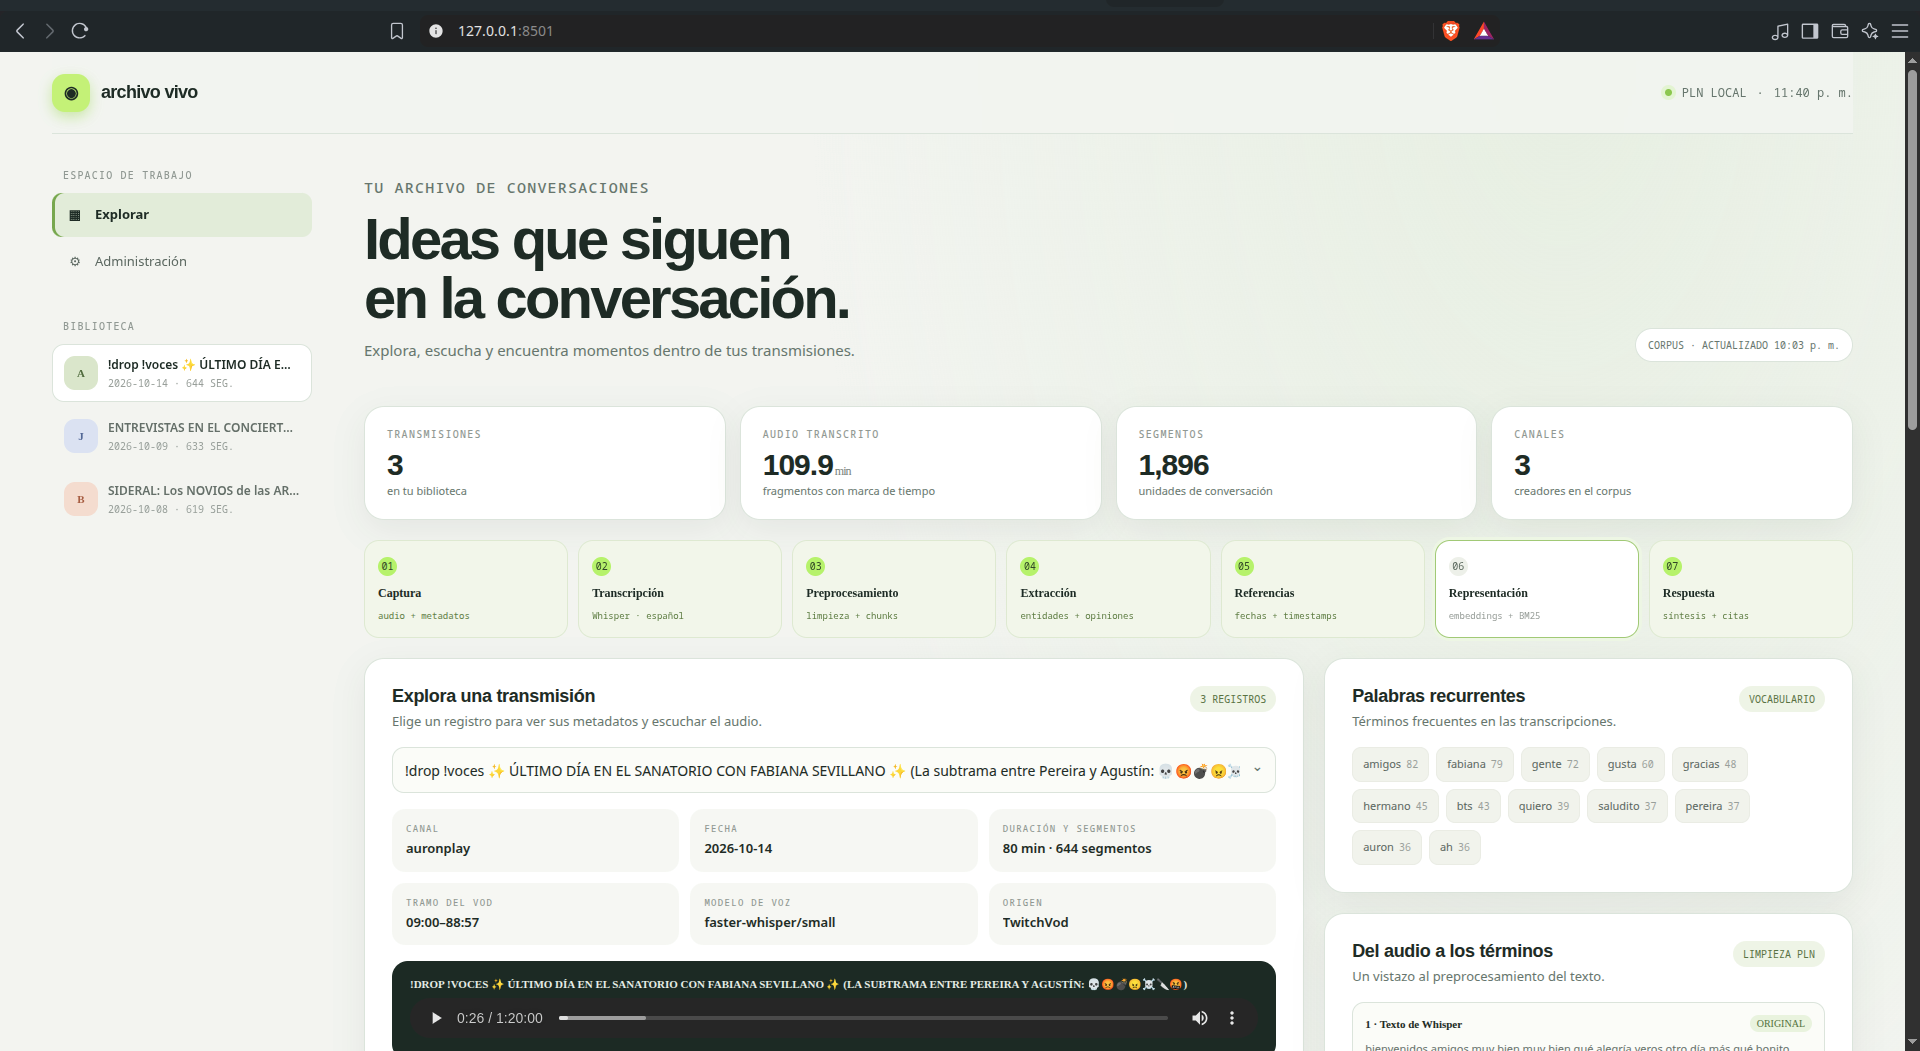
\includegraphics[width=0.95\linewidth]{image.png}
  \caption{Interfaz web del prototipo. Pestaña \emph{Explorar}: resumen del corpus, reproductor de audio con salto por marca temporal y panel de consulta en lenguaje natural.}
  \label{fig:interfaz}
\end{figure}

La \emph{API} expone los siguientes servicios principales:

\begin{table}[h]
\centering
\small
\begin{tabular}{@{}llp{7.4cm}@{}}
\toprule
\textbf{Método} & \textbf{Ruta} & \textbf{Función} \\
\midrule
GET  & \texttt{/api/transmissions}     & Lista de transmisiones y estadísticas del corpus. \\
GET  & \texttt{/api/memory/<id>}       & Memoria completa de una transmisión. \\
GET  & \texttt{/api/creator-memory/<k>}& Memoria agrupada por creador. \\
GET  & \texttt{/media/<id>}            & Audio con soporte de peticiones parciales. \\
POST & \texttt{/api/ask}               & Pregunta en lenguaje natural (con intención y filtros). \\
POST & \texttt{/api/process}           & Ingesta de un enlace nuevo. \\
POST & \texttt{/api/process-memory}    & Construye la memoria de una transcripción. \\
POST & \texttt{/api/retranscribe}      & Compara un modelo de Whisper. \\
GET  & \texttt{/api/evaluation}        & Precision@$K$ y Recall@$K$ actuales. \\
\bottomrule
\end{tabular}
\caption{Servicios principales de la API local.}
\label{tab:api}
\end{table}

% ---------------------------------------------------------------------------

\section{Diseño de la Interfaz y Experiencia de Usuario}
\label{sec:ux}

El objetivo de la interfaz es que el usuario perciba el sistema como una extensión de su propia memoria: pregunta como preguntaría a un asistente y recibe una respuesta que puede verificar. Para lograrlo, el diseño se guió por tres principios. El primero es la claridad: la pantalla debe comunicar de inmediato qué contiene el corpus y cómo formular una consulta. El segundo es la verificabilidad: toda respuesta debe poder comprobarse con un solo clic. El tercero es la autonomía: el usuario avanzado debe poder gestionar el corpus sin depender del desarrollador.

La pantalla de exploración presenta en primer lugar un resumen del corpus con el número de transmisiones, los minutos procesados, el total de segmentos y los canales disponibles. Este resumen cumple una función de orientación: sitúa al usuario antes de que formule su primera pregunta. Debajo aparece la lista de transmisiones con sus metadatos, un reproductor de audio con salto directo a la marca temporal, el contador de palabras y los términos recurrentes. Así, la evidencia deja de ser una promesa abstracta y se convierte en una posición concreta del audio.

El panel de consulta acepta preguntas en lenguaje natural y muestra la respuesta redactada junto con sus referencias. Cada referencia incluye el creador, la transmisión y el minuto exacto, de modo que el usuario puede abrir el video original en ese instante. Cuando la consulta no encuentra evidencia suficiente, el sistema lo indica con claridad en lugar de fabricar una respuesta. Esta postura, poco habitual en herramientas que premian la apariencia de completitud, refuerza la confianza a largo plazo.

La sección de administración completa el ciclo del usuario avanzado. Permite agregar un enlace nuevo con sus parámetros, volver a obtener el audio, borrar o eliminar registros, comparar distintos tamaños de modelo de reconocimiento sobre el mismo archivo, activar una transcripción revisada manualmente, construir la memoria y explorar el grafo de relaciones, las entidades detectadas y el panel de evaluación. La separación en dos espacios —consulta y gestión— mantiene la sencillez de la vista principal. El minimalismo visual, la respuesta humanizada y la cita compacta sirven a este propósito; la captura de la Figura~\ref{fig:interfaz} documenta el estado actual de la interfaz.


\section{Metodología de Desarrollo}
\label{sec:metodologia}

El desarrollo siguió cuatro fases incrementales, coherentes con la propuesta original:

\begin{enumerate}
  \item \textbf{Recolección y limpieza.} Elección de las transmisiones, descarga de los tramos de audio, transcripción con Whisper y formato de segmentos con metadatos de tiempo.
  \item \textbf{Construcción del \emph{pipeline} PLN.} Normalización, separación de \emph{stopwords} por categoría, protección de fechas, segmentación, NER, opiniones, relaciones, referencias temporales y contador de palabras.
  \item \textbf{Representación e indexado.} Generación de \emph{embeddings} multilingües y recuperación híbrida (BM25 + similitud densa) con filtrado por metadatos y por tiempo.
  \item \textbf{Respuesta, interfaz y validación.} Redacción de respuestas con cita compacta, generación RAG opcional, interfaz web y verificación cualitativa con preguntas de prueba sobre el corpus.
\end{enumerate}

% ---------------------------------------------------------------------------

\section{Ingeniería del Software, Arquitectura y Despliegue}
\label{sec:ingenieria}

Más allá de los algoritmos de PLN, el prototipo es un artefacto de software que debe ser comprensible, modificable y reproducible. Esta sección describe las decisiones de ingeniería que sostienen el sistema, desde su organización modular hasta las consideraciones de seguridad, rendimiento y portabilidad.

\subsection{Organización modular y separación de responsabilidades}

El código se organiza en cuatro capas con responsabilidades bien delimitadas. La capa de \emph{ingesta} se encarga de obtener el audio y transcribirlo; la capa de \emph{PLN} transforma el texto en la memoria semántica; la capa de \emph{consulta} recupera evidencia y compone la respuesta; y la capa de \emph{interfaz} expone el sistema al usuario mediante una página web y una API local. Esta separación permite reemplazar una capa sin reescribir las demás; por ejemplo, se puede sustituir el modelo de reconocimiento de voz o el motor de recuperación sin tocar la interfaz. La modularidad también facilita las pruebas: cada componente puede ejercitarse de forma aislada.

\subsection{Elección deliberada de dependencias mínimas}

Una decisión de diseño fue evitar \emph{frameworks} pesados. La interfaz se sirve con la biblioteca estándar de Python y HTML, sin dependencias de servidores de aplicaciones ni de herramientas de construcción de front-end. El resultado es un sistema que se instala con pocos paquetes, arranca en segundos y puede ejecutarse íntegramente en un equipo personal. Esta austeridad no es solo una preferencia estética: reduce los puntos de fallo, facilita la auditoría del código y hace viable la ejecución en entornos con recursos limitados, como el aula o un portátil sin GPU.

\subsection{Ejecución local y eficiencia en CPU}

El reconocimiento de voz es la etapa más costosa. Para hacerlo viable sin aceleración por hardware, se utilizó una implementación optimizada con cuantización a enteros de 8 bits, que reduce el uso de memoria y acelera la inferencia en CPU con una pérdida mínima de precisión. El sistema ofrece distintos tamaños de modelo, de modo que el usuario puede elegir entre velocidad y calidad; los modelos pequeños son útiles para pruebas rápidas, mientras que los medianos ofrecen una transcripción más fiel. Los resultados de cada corrida se conservan con un identificador de modelo, lo que permite comparar salidas y auditar qué modelo produjo cada transcripción.

\subsection{Reproducibilidad y trazabilidad}

La reproducibilidad es un requisito explícito del proyecto. Cada artefacto derivado —audio, transcripción, memoria y resultado de evaluación— se guarda en disco con nombres predecibles y metadatos que registran su procedencia. Las corridas de modelo se almacenan por separado, de manera que sea posible volver a generar cualquier salida o comparar versiones. El sistema también admite activar una transcripción revisada manualmente, conservando una copia de respaldo de la versión automática original. Este cuidado convierte el prototipo en una herramienta de investigación y no solo en una demostración.

\subsection{Seguridad, privacidad y despliegue}

El sistema funciona en local y no requiere credenciales en la nube. La API se limita a operaciones sobre el propio corpus y no expone datos personales del chat ni de terceros. El servidor de medios implementa soporte de peticiones parciales, lo que permite buscar dentro de un audio largo sin descargarlo completo y mejora la experiencia de reproducción. Para un despliegue en red, bastaría añadir autenticación y cifrado, pero el diseño actual prioriza la sencillez y la transparencia por tratarse de un prototipo académico. Estas consideraciones se retoman en la sección de ética y en el trabajo futuro.


\section{Resultados con el Corpus}
\label{sec:resultados}

Sobre la transmisión \texttt{v2900590088} (auronplay, 9--80~min) se construyó la memoria persistente cuyos recuentos se resumen en la Tabla~\ref{tab:memoria}. Los \emph{embeddings} quedaron en estado \texttt{ready} con el modelo multilingüe, y la memoria conserva el esquema 4 y el índice de búsqueda versión 4.

\begin{table}[h]
\centering
\small
\begin{tabular}{@{}lr@{}}
\toprule
\textbf{Elemento de la memoria} & \textbf{Cantidad} \\
\midrule
Fragmentos (\emph{chunks}) & 247 \\
Entidades candidatas & 43 \\
Relaciones explícitas & 4 \\
Opiniones candidatas & 21 \\
Referencias temporales & 90 \\
Palabras totales & 10\,628 \\
Palabras de contenido & 3\,258 \\
Palabras únicas de contenido & 1\,521 \\
Diversidad léxica & 0{,}467 \\
\emph{Embeddings} & \texttt{ready} \\
\bottomrule
\end{tabular}
\caption{Resumen de la memoria construida para \texttt{v2900590088}.}
\label{tab:memoria}
\end{table}

La búsqueda devuelve fragmentos con una idea completa y una cita reproducible. Por ejemplo, ante una pregunta sobre «Fabiana», el sistema localiza el momento exacto, redacta la postura del creador y muestra el enlace al minuto correspondiente del VOD. Los términos más frecuentes de contenido (por ejemplo, «fabiana», «pereira», «tiktok») orientan la lectura del corpus sin confundir muletillas con temas.

La Tabla~\ref{tab:compara} contrapone los dos modos del recuperador, que se activan según la disponibilidad de \emph{embeddings}.

\begin{table}[h]
\centering
\small
\begin{tabular}{@{}lll@{}}
\toprule
\textbf{Modo} & \textbf{Señal} & \textbf{Comportamiento} \\
\midrule
Línea base & BM25 & Siempre disponible, rápida, léxica. \\
Híbrido    & BM25 + coseno & Requiere \emph{embeddings}; captura paráfrasis y sinónimos. \\
\bottomrule
\end{tabular}
\caption{Modos de recuperación del prototipo.}
\label{tab:compara}
\end{table}

% ---------------------------------------------------------------------------

\section{Casos de Estudio y Ejemplos de Consulta}
\label{sec:casos}

La mejor forma de entender el comportamiento del sistema es observar consultas reales sobre el corpus. A continuación se describen varios escenarios representativos, el tipo de procesamiento que activan y el aspecto de la respuesta obtenida. Estos ejemplos ilustran cómo convergen las distintas técnicas de PLN en una experiencia de uso concreta.

\subsection{Consulta sobre una persona}

Cuando el usuario pregunta qué se dijo sobre una persona concreta, el sistema reconoce en la pregunta una entidad de tipo persona mediante el modelo de NER. Esa entidad se usa como filtro: se privilegian los fragmentos en los que aparece la misma persona y se ordenan por relevancia léxica y semántica. La respuesta resultante cita al creador, el minuto del directo y la frase exacta en la que se menciona a la persona. Este escenario demuestra la utilidad combinada del reconocimiento de entidades y de la cita temporal: sin el primero, la búsqueda sería lexical y ruidosa; sin el segundo, la respuesta no sería verificable.

\subsection{Consulta de opinión}

Si la pregunta utiliza verbos como ``opina'', ``piensa'' o ``le gusta'', el sistema infiere la intención de opinión y busca no solo menciones, sino tripletas de opinión previamente extraídas. La respuesta incorpora entonces una valoración de polaridad —positiva o negativa— y la evidencia textual que la sustenta. Este caso muestra por qué el análisis de sentimiento agrega valor: el usuario no solo obtiene el fragmento donde aparece un tema, sino la actitud del creador frente a él, algo que una búsqueda por palabras clave jamás revelaría.

\subsection{Consulta temporal}

Las preguntas que contienen expresiones como ``al inicio'', ``al final'' o ``en el minuto cuarenta'' activan el filtro temporal. El sistema normaliza esas expresiones, las convierte en un rango de segundos y restringe la recuperación a los fragmentos que caen dentro de ese rango. Gracias a la protección de las fechas y las referencias temporales durante la normalización, el filtro no se rompe por la eliminación de tildes ni por la tokenización. Este escenario ilustra la importancia de tratar las expresiones temporales como ciudadanos de primera clase del sistema, y no como palabras vacías descartables.

\subsection{Consulta sobre temas recurrentes}

Cuando el usuario pregunta de qué se habló más, el sistema recurre al vocabulario de contenido —términos frecuentes una vez descartadas las palabras funcionales— y resume los temas dominantes, citando un fragmento representativo de cada uno. Esta vista es especialmente útil para obtener un panorama rápido de una transmisión larga antes de profundizar en un aspecto concreto. El contador de palabras y el cálculo de riqueza léxica complementan esta función al ofrecer una medida objetiva del vocabulario empleado.

\subsection{Consulta entre transmisiones}

El sistema permite agrupar la memoria por creador, de modo que una consulta pueda comparar varias transmisiones del mismo canal. Así, es posible preguntar por la evolución de un tema a lo largo del tiempo o por la coincidencia de opiniones entre distintos directos. Este escenario anticipa el uso del prototipo como herramienta de seguimiento, y motiva el trabajo futuro sobre agregación y resumen multi-documento.

\subsection{Consulta sin evidencia suficiente}

Un comportamiento honesto, y a menudo olvidado, es el de la consulta que no tiene respuesta en el corpus. Cuando la evidencia recuperada es insuficiente, el sistema debe admitirlo en lugar de inventar. Esta decisión, reforzada por las restricciones del modo RAG, protege la confianza del usuario y distingue a un sistema de recuperación de un generador de texto libre. Documentar este caso es tan importante como documentar los aciertos, porque delimita el alcance real de la herramienta.



\section{Calidad de Datos, Anotación y Sesgos}
\label{sec:calidad}

La calidad de una memoria semántica depende de la calidad de sus fuentes. En este proyecto la fuente primaria es una transcripción automática y, por tanto, hereda sus imperfecciones: palabras mal reconocidas, nombres propios deformados, puntuación ausente y fronteras de oración imprecisas. Reconocer estas limitaciones es el primer paso para mitigarlas; el segundo es ofrecer al usuario la posibilidad de revisar y corregir la transcripción sin perder la versión original.

La anotación es el segundo pilar de la calidad. Las métricas de recuperación requieren un conjunto de preguntas con respuestas relevantes señaladas manualmente, conocido como conjunto dorado. Construirlo exige una guía de anotación explícita, con criterios y ejemplos, y una revisión que reduzca la subjetividad. La validez de cualquier número reportado depende de ese esfuerzo previo, habitualmente subestimado.

Los sesgos merecen atención particular. Un corpus formado por unas pocas transmisiones de unos pocos creadores refleja sus temas, su vocabulario y sus intereses, no los de la población general. Las entidades reconocidas, las opiniones extraídas y los temas frecuentes heredan ese sesgo de selección. Del mismo modo, un modelo de voz entrenado con ciertos acentos puede transcribir peor a hablantes de otras variedades, generando una desventaja sistemática. Documentar estas asimetrías es imprescindible para no presentar generalizaciones indebidas.

Un sesgo más sutil es el de la normalización: al eliminar tildes o al filtrar palabras frecuentes, el sistema puede borrar diferencias dialectales o de registro. La decisión de conservar el texto original en la memoria, separado del texto de búsqueda, mitiga este riesgo, porque aunque la búsqueda simplifique, la evidencia preserva la forma original. En última instancia, la trazabilidad es la mejor defensa: si cada dato puede rastrearse hasta su fragmento y su segundo exactos, el usuario queda en condiciones de juzgar por sí mismo la fiabilidad de lo que el sistema afirma.


\section{Evaluación}
\label{sec:evaluacion}

La evaluación se diseñó en dos frentes complementarios: la calidad de la transcripción (ASR) y la calidad de la recuperación.

\subsection{Evaluación del reconocimiento de voz}

Se implementó una utilidad en Administración que transcribe el mismo MP3 con distintos tamaños de Whisper y guarda las salidas en \texttt{data/processed/model\_runs/} sin sustituir la transcripción activa. Así se comparan \texttt{small} y \texttt{medium} sobre el mismo audio. La limitación honesta es que la comparación ideal exige una transcripción de referencia corregida manualmente; por ahora la revisión es cualitativa sobre una muestra. En este equipo, sin aceleración por GPU disponible, la inferencia corre en CPU con \texttt{int8}, lo que hace lenta la retranscripción de VOD largos.

\subsection{Evaluación de la recuperación}

El proyecto incluye \texttt{src/nlp/evaluate\_retrieval.py}, que calcula \textbf{Precision@$K$} y \textbf{Recall@$K$} contra un conjunto de preguntas y rangos anotados manualmente en \texttt{data/evaluation/gold\_questions.jsonl}. La lógica considera acierto cuando un fragmento recuperado en los primeros $K$ resultados se solapa con un rango de referencia para la misma transmisión.


\textbf{Estado actual.} El conjunto de preguntas de referencia aún debe completarse con al menos diez preguntas variadas (tema, opinión, recomendación, referencia temporal y búsqueda general) y sus rangos de tiempo reales, revisados escuchando el audio. Por eso no se declaran todavía valores de Precision@5 ni Recall@5 como resultado definitivo: reportar métricas sobre un conjunto vacío sería metodológicamente incorrecto. La herramienta y el flujo de anotación ya están listos para completar esa etapa.

\subsection{Revisión cualitativa}

Se verificó que las respuestas citan el fragmento correcto y que el enlace abre el VOD en el minuto indicado. Los cambios más notables respecto de versiones anteriores fueron: las opiniones dejaron de estar en cero al pasar el modelo a la extracción, las entidades espurias (muletillas, interjecciones) se redujeron drásticamente con la validación, y las fechas dejaron de romperse al eliminar \emph{stopwords}.

% ---------------------------------------------------------------------------

\section{Análisis Comparativo con Alternativas Existentes}
\label{sec:comparacion}

Para valorar el aporte del prototipo conviene compararlo con las alternativas que un usuario tendría a mano. La Tabla~\ref{tab:comparacion} resume la comparación en dimensiones clave: la capacidad de buscar por contenido hablado, la de responder preguntas en lenguaje natural, la de citar la evidencia y la de ofrecer estructura semántica.

\begin{table}[h]
\centering
\small
\begin{tabular}{@{}p{3.5cm}p{2.4cm}p{2.4cm}p{2.4cm}p{3.2cm}@{}}
\toprule
\textbf{Alternativa} & \textbf{Búsqueda por voz} & \textbf{Preguntas NL} & \textbf{Cita con tiempo} & \textbf{Estructura semántica} \\
\midrule
Búsqueda de la plataforma & No & No & No & No \\
Ver el video completo & Sí (manual) & No & Imprecisa & No \\
Transcripción plana & A veces & No & Por línea & No \\
Servicios de transcripción & Sí & Parcial & Parcial & Limitada \\
Asistente general sobre el texto & Sí & Sí & A veces & Limitada \\
\textbf{Este prototipo} & Sí & Sí & Sí & Entidades, relaciones y opiniones \\
\bottomrule
\end{tabular}
\caption{Comparación cualitativa entre alternativas de acceso a contenido hablado.}
\label{tab:comparacion}
\end{table}

La búsqueda nativa de las plataformas indexa metadatos, no lo que se dice. Ver el video completo es la única forma de recuperar una mención concreta, pero exige un tiempo desproporcionado. Una transcripción plana permite buscar palabras, aunque no entiende el significado ni distingue opiniones de hechos. Los servicios de transcripción añaden subtítulos, pero rara vez estructuran entidades y relaciones. Los asistentes generales pueden responder preguntas sobre un texto transcrito, aunque sin garantizar que la respuesta esté anclada a un instante verificable del audio.

Frente a ellos, el prototipo integra las capacidades en un único flujo local: recupera por significado y por léxico, reconoce entidades, extrae opiniones, respeta el orden temporal y, sobre todo, cita cada respuesta con el creador, la transmisión y el minuto exactos. Esa combinación es la que convierte una transcripción en una memoria consultable y confiable. Reconocer las limitaciones —escala pequeña, evaluación cuantitativa incompleta, dependencia de la calidad del ASR— es parte de una comparación honesta, pero también define con claridad el valor diferencial de la propuesta.



\section{Preguntas de Investigación y Validación}
\label{sec:preguntas}

Todo trabajo de investigación se ordena en torno a preguntas que guían el diseño y la evaluación. Este proyecto se articula alrededor de cuatro preguntas centrales, cada una con un criterio de validación asociado.

La primera pregunta indaga si es posible construir, con herramientas de PLN accesibles y ejecutables en un equipo personal, una memoria semántica que represente el contenido hablado de forma estructurada. La validación es funcional: la memoria debe contener fragmentos, entidades, relaciones, opiniones y referencias temporales coherentes con el corpus, y debe ser capaz de responder consultas. Los resultados sobre el corpus real confirman esta viabilidad.

La segunda pregunta se refiere a si la recuperación híbrida, que combina coincidencia léxica y similitud semántica, supera a cada señal por separado. La validación rigurosa exige un conjunto de preguntas con respuestas relevantes anotadas y el cálculo de Precision@K y Recall@K. El sistema ya implementa estas métricas, pero el conjunto de anotación permanece vacío, por lo que la respuesta queda planteada como hipótesis y su comprobación se traslada al trabajo futuro. Declararlo así es una forma de honestidad metodológica.

La tercera pregunta aborda si la respuesta con cita verificable mejora la utilidad percibida por el usuario frente a una lista de fragmentos crudos. La validación se apoya en la revisión cualitativa de casos de estudio: se observa si la respuesta es comprensible, si la cita es correcta y si el usuario puede comprobar la evidencia con un solo clic. Los ejemplos de la sección anterior respaldan esta mejora cualitativa.

La cuarta pregunta explora las limitaciones y los desafíos que emergen al aplicar PLN a habla espontánea de plataformas de \emph{streaming}: errores de transcripción, jerga, solapamiento de voces y ambigüedad. La validación es descriptiva y honesta: se documentan los fallos observados y se proponen mitigaciones. Esta pregunta reconoce que un prototipo académico no resuelve todos los problemas, sino que los hace visibles y trazables.

Establecer preguntas y criterios de validación explícitos tiene una ventaja adicional: convierte el proyecto en un programa de investigación con pasos siguientes claros, en lugar de una demostración cerrada.



\section{Métricas de Evaluación en Detalle}
\label{sec:metricas}

Una discusión rigurosa exige precisar qué mide cada métrica y por qué se elige. La tasa de error de palabras (WER) compara la transcripción con una referencia humana y cuenta sustituciones, inserciones y eliminaciones; su valor se interpreta como el porcentaje de palabras incorrectas. La tasa de error de caracteres (CER) es análoga pero opera a nivel de carácter, útil cuando la segmentación en palabras es ambigua. Ambas permiten cuantificar la calidad del reconocimiento de voz y localizar en qué tipo de habla falla más el modelo.

En recuperación, la precisión en los primeros K resultados (Precision@K) indica qué fracción de los K fragmentos devueltos es relevante, mientras que la exhaustividad (Recall@K) indica qué proporción del total de fragmentos relevantes quedó dentro de esos K. Estas dos métricas suelen oponerse: aumentar K mejora la exhaustividad a costa de la precisión. Para resumir el comportamiento en distintos valores de K, se emplean la precisión media promedio (MAP) y la ganancia acumulada descontada normalizada (nDCG), que premian colocar los aciertos en las primeras posiciones.

Para la generación de texto se emplean ROUGE y BLEU, basadas en el solapamiento de n-gramas con referencias humanas. En un sistema con cita, sin embargo, estas métricas son limitadas: una respuesta puede ser distinta en redacción y aun así correcta, o parecida y aun así infundada. Por eso se complementa la medición automática con la verificación de que cada afirmación esté respaldada por la evidencia citada.

En este trabajo, el sistema ya implementa el cálculo de Precision@K y Recall@K, pero el conjunto de preguntas anotado permanece vacío, por lo que no se reportan cifras. Hacer explícita esta ausencia, en lugar de presentar números no reproducibles, es coherente con el principio de honestidad metodológica que atraviesa el informe.



\section{Consideraciones sobre la Calidad de la Respuesta}
\label{sec:calidadresp}

La calidad de una respuesta en lenguaje natural depende de varios factores que conviene distinguir. El primero es la relevancia: el fragmento recuperado debe corresponder realmente a lo que se preguntó. El segundo es la fidelidad: la respuesta no debe afirmar nada que la evidencia no respalde. El tercero es la claridad: la redacción debe ser comprensible para una persona que no conoce los detalles técnicos. El cuarto es la verificabilidad: el usuario debe poder comprobar la afirmación con facilidad. Un sistema que acierta en relevancia pero falla en fidelidad resulta peligroso; uno que es fiel pero oscuro resulta inútil.

La respuesta extractiva del prototipo se diseñó para equilibrar estos factores. Al construir una o dos frases que introducen el fragmento más informativo y lo cierran con una cita compacta, se busca claridad y verificabilidad sin renunciar a la fidelidad, porque el texto proviene directamente de la evidencia. La cita incluye creador, transmisión y minuto, de modo que la comprobación exige un solo clic. Este diseño evita la sensación de caja negra que a menudo acompaña a los asistentes automáticos.

El modo de generación aumenta la fluidez a costa de un riesgo adicional de infidelidad. Por eso se acota con restricciones estrictas y se descarta su salida si no cita la evidencia. El equilibrio entre naturalidad y fidelidad es, en el fondo, un problema de confianza: el usuario debe poder confiar en que lo que lee corresponde a lo que se dijo. En ese sentido, la cita no es un adorno, sino la garantía central del sistema. Mejorar la calidad de la respuesta implica, por tanto, mejorar simultáneamente la recuperación, la redacción y la cita, sin sacrificar ninguna de las tres.


\section{Discusión y Limitaciones}
\label{sec:limitaciones}

El prototipo funciona de extremo a extremo, pero es importante declarar sus límites con honestidad:

\begin{itemize}
  \item \textbf{Transcripción no perfecta.} Whisper \texttt{medium} no garantiza nombres propios correctos; se requiere revisión humana de una muestra antes de tratar el texto como exacto.
  \item \textbf{Señales candidatas.} NER, relaciones y opiniones son \emph{candidatas} basadas en reglas; el sistema no comprende ironía, citas ni negación compleja y no debe presentar sus aristas como hechos confirmados.
  \item \textbf{Sin diarización.} No se distingue quién habla cuando participan varias personas; el sistema no infiere identidad por la voz.
  \item \textbf{Referencias relativas.} La detección temporal por expresiones regulares no resuelve todas las referencias relativas a una fecha absoluta ni la correferencia temporal.
  \item \textbf{Recuperación en memoria.} Para el corpus pequeño se recorre el índice en memoria; no hay una base vectorial escalable del tipo FAISS/Chroma, aunque el diseño lo permitiría.
  \item \textbf{Generación opcional.} Sin un LLM local configurado, la respuesta es extractiva. El modo RAG existe pero no se ha demostrado una mejora medida frente a la línea base.
\end{itemize}

Estas limitaciones no invalidan el prototipo: delimitan con precisión qué puede afirmarse y preparan el camino para las siguientes fases.

% ---------------------------------------------------------------------------

\section{Síntesis de Hallazgos y Contribuciones}
\label{sec:sintesis}

Reunidos los resultados, conviene sintetizar qué se aprendió y qué aporta este trabajo. El primer hallazgo es que la separación de responsabilidades en el preprocesamiento —listas de palabras vacías distintas para búsqueda y contenido, y protección explícita de fechas y negaciones— mejora de forma tangible la calidad de la recuperación. Tratar todas las palabras vacías por igual, como suele hacerse, destruye matices esenciales; tratarlas con criterio los preserva.

El segundo hallazgo es que el enriquecimiento semántico con entidades, opiniones y relaciones transforma la naturaleza de la experiencia. La transcripción deja de ser un muro de texto y se convierte en una base navegable donde las preguntas encuentran respuestas respaldadas por evidencia. El reconocimiento de entidades con validación de dominio resultó especialmente importante para filtrar el ruido introducido por el ASR.

El tercer hallazgo es que la cita temporal es la característica que más acerca el sistema a las expectativas del usuario. Poder saltar al segundo exacto del video convierte una respuesta abstracta en una prueba concreta y verificable. Esta característica depende de que las marcas temporales se conserven desde la transcripción hasta la respuesta, lo que refuerza la importancia de no perderlas en ninguna etapa.

La contribución principal del proyecto es un prototipo funcional, abierto y reproducible que integra reconocimiento de voz, procesamiento de lenguaje natural, recuperación híbrida y generación acotada en un único flujo local. A diferencia de soluciones cerradas, el sistema es auditable de principio a fin: el código, los datos y las decisiones están disponibles para su revisión. Este carácter abierto es, en un contexto académico, tanto un aporte como una garantía.

La segunda contribución es metodológica. El informe documenta con honestidad lo que se logró y lo que no: la evaluación cuantitativa queda pendiente, el conjunto de anotación está vacío y algunas limitaciones de escala persisten. Lejos de restar valor, esta transparencia establece una línea base sobre la cual otros pueden construir y medir avances. Una contribución que se reconoce a sí misma sus límites es más útil que una que los oculta.

Finalmente, el trabajo aporta una demostración de que las técnicas de PLN, incluso en su versión más accesible y sin recursos de nube, permiten rescatar el conocimiento atrapado en el habla y ponerlo al servicio de las personas. Esa es, en el fondo, la contribución que da sentido al esfuerzo.



\section{Amenazas a la Validez del Estudio}
\label{sec:validez}

Ningún estudio está exento de limitaciones que amenacen la validez de sus conclusiones, e identificarlas explícitamente es una práctica de rigor. Pueden agruparse en cuatro categorías. Las amenazas de constructo se refieren a si lo que se mide corresponde al concepto que se pretende medir; aquí, la calidad de la memoria se evalúa de forma cualitativa y la calidad de la recuperación no llega a medirse con un conjunto dorado, de modo que existe el riesgo de no capturar del todo la utilidad real para el usuario.

Las amenazas internas aluden a las relaciones causales. Afirmar que la recuperación híbrida supera a cada señal por separado exigiría un experimento controlado que este trabajo no completó; por tanto, tal afirmación se mantiene como hipótesis y no como resultado. Del mismo modo, los ejemplos de consulta se eligieron para ilustrar capacidades y no constituyen una muestra aleatoria. Las amenazas externas, por su parte, tienen que ver con la generalización: el corpus es pequeño, de un solo idioma y de unos pocos creadores, por lo que los resultados no se extrapolan sin más a otros dominios, idiomas o escalas.

Finalmente, las amenazas de conclusión estadística derivan del tamaño de la muestra. Sin un conjunto de evaluación amplio no cabe hacer inferencias con intervalos de confianza ni pruebas de significación. Lo que sí puede afirmarse con seguridad es la viabilidad técnica del flujo completo y la utilidad cualitativa de la respuesta con cita. Reconocer estas amenazas no debilita el trabajo: lo sitúa con precisión y traza el camino para reforzarlo en el futuro.



\section{Reflexiones sobre la Evaluación con Usuarios}
\label{sec:evalusuarios}

La evaluación de un sistema de recuperación no se agota en las métricas automáticas. Al final, lo que importa es si un usuario real encuentra lo que busca y confía en lo que obtiene. La evaluación con personas, aunque costosa, aporta una perspectiva que ninguna cifra sustituye. En un prototipo de este tipo, un estudio de usuarios permitiría medir la satisfacción, el tiempo hasta la respuesta útil y la confianza en la cita.

Un diseño razonable de estudio pediría a los participantes formular preguntas sobre un corpus que desconocen y luego valorar la utilidad y la corrección de cada respuesta en una escala. Se registraría el tiempo empleado, si el usuario abre la referencia y si considera que la cita respalda la respuesta. Estas señales, más cualitativas que el Precision@K, capturan dimensiones como la confianza y la claridad, difíciles de reducir a un número.

Un aspecto delicado es la comparación honesta. Si se comparara la respuesta humanizada con una lista de fragmentos crudos, habría que controlar el orden, la presentación y el tiempo, y evitar que el entusiasmo por la novedad sesgue la valoración. Idealmente, se compararían también un asistente de propósito general y la búsqueda nativa de la plataforma, para situar la contribución en un contexto realista.

Finalmente, la evaluación con usuarios permite descubrir problemas invisibles para las métricas: consultas ambiguas que el sistema interpreta mal, respuestas técnicamente correctas pero confusas, o citas que el usuario no sabe cómo interpretar. Incorporar estos hallazgos al diseño es una de las lecciones más valiosas que puede dejar un prototipo. Este trabajo no llega a ejecutar tal estudio, pero deja planteado su diseño porque reconoce su importancia para validar la utilidad real del sistema.


\section{Conclusiones}
\label{sec:conclusiones}

El trabajo demuestra la viabilidad técnica de construir memorias semánticas inteligentes aplicadas a medios digitales. Los principales aprendizajes y logros fueron:

\begin{itemize}
  \item Separar \texttt{SEARCH\_STOPWORDS} y \texttt{CONTENT\_STOPWORDS} y proteger las fechas eliminó el sesgo de la negación y evitó romper referencias temporales.
  \item El NER con validación y vocabulario de dominio mejora de forma notable la limpieza de entidades.
  \item Pasar el modelo de lenguaje a la extracción de opiniones habilitó su detección (de 0 a decenas según la transmisión).
  \item La respuesta humanizada con cita compacta deja de sentirse como un buscador: entrega prosa natural y evidencia verificable.
  \item La recuperación híbrida y el contador de palabras añaden utilidad práctica sin complejidad innecesaria.
  \item La integración de herramientas de PLN (entidades, sentimiento, búsqueda vectorial) transforma horas de transmisiones informales en una fuente de conocimiento interactiva y estructurada, resolviendo la dispersión de información en las plataformas de streaming.
\end{itemize}

% ---------------------------------------------------------------------------

\section{Impacto Social, Económico y Cultural}
\label{sec:impacto}

Las implicaciones de un sistema capaz de convertir contenido hablado en conocimiento consultable trascienden lo técnico. En el plano social, facilita el acceso a información que hoy es prácticamente inaccesible para personas con discapacidad auditiva, para quienes la transcripción estructurada y la búsqueda por contenido abren una puerta al contenido audiovisual. También favorece la inclusión lingüística al permitir consultar en lenguaje natural sin conocer términos exactos.

En el plano educativo, un sistema de este tipo puede transformar clases, seminarios y conferencias en materiales navegables. En lugar de revisar horas de grabación, el estudiante o el docente formula una pregunta y accede al fragmento relevante. La misma lógica se aplica a la investigación periodística, donde verificar una declaración dicha al aire es una necesidad constante; una memoria semántica con cita temporal reduce drásticamente el tiempo de verificación y refuerza la trazabilidad de las fuentes.

En el plano económico, los creadores de contenido y las empresas de medios pueden explotar mejor su propio archivo. Un catálogo de transmisiones convertido en memoria semántica habilita recomendaciones, resúmenes automáticos y búsquedas internas que hoy no existen o dependen de trabajo manual. Para negocios pequeños, la posibilidad de ejecutar la herramienta en un equipo personal, sin costos de nube, democratiza una capacidad reservada a grandes plataformas.

En el plano cultural, el habla espontánea es una forma de patrimonio poco documentada. Las conversaciones, la jerga y las opiniones registradas en transmisiones en vivo constituyen una huella de su época. Preservarlas de forma estructurada y consultable contribuye a su conservación y estudio. Naturalmente, este potencial exige un marco ético cuidadoso, que respete la autoría del contenido y el derecho a la privacidad, aspectos tratados en la sección correspondiente.

Estos impactos, presentes incluso en un prototipo modesto, explican por qué el problema merece atención académica y por qué las herramientas de PLN son un instrumento adecuado para abordarlo.



\section{Escalabilidad y Costos Computacionales}
\label{sec:escalabilidad}

La técnica desarrollada debe proyectarse más allá de un corpus pequeño. La escalabilidad del sistema depende de cuatro factores: el volumen de datos, el costo del reconocimiento de voz, el cálculo de representaciones vectoriales y la recuperación. El reconocimiento de voz es la etapa dominante: su costo crece con la duración del audio, y procesar muchas horas exige paralelizar la ingesta, algo natural porque cada tramo es independiente. Para hacerlo viable sin aceleración por hardware se empleó una implementación optimizada con cuantización de enteros, que reduce el uso de memoria y acelera la inferencia en CPU con una pérdida mínima de precisión.

Las etapas de PLN y de representación vectorial son más económicas. La extracción de entidades, opiniones y relaciones recorre el texto una vez, y el cálculo de representaciones puede organizarse por lotes. Cuando la colección crece, la búsqueda exacta sobre todos los vectores deja de ser viable y se recurre a índices de vecinos más cercanos aproximados, como los basados en grafos o en cuantización; el diseño modular contempla esa migración sin reescribir el resto del sistema.

En términos de despliegue, ejecutar todo en local elimina los costos recurrentes de la nube y refuerza la privacidad, a cambio de mayor tiempo de cómputo. Para un usuario individual, un aula o una pequeña organización, ese intercambio es favorable. Para volúmenes muy grandes, en cambio, conviene evaluar el uso de hardware especializado y de almacenamiento dedicado. En ambos extremos, el criterio de diseño permanece constante: preservar la trazabilidad y la capacidad de auditar cada resultado, sin sacrificar la calidad por la escala.



\section{Aplicaciones Potenciales y Escenarios de Adopción}
\label{sec:aplicaciones}

La técnica desarrollada habilita aplicaciones que trascienden el caso de estudio. Un primer escenario es el archivo personal de un creador de contenido que desea ofrecer a su audiencia una búsqueda por lo que dijo a lo largo de años de transmisiones; la memoria semántica funcionaría como índice interno que responde preguntas y enlaza al momento exacto. Un segundo escenario es el educativo: convertir clases y conferencias grabadas en materiales consultables, con búsqueda por concepto y respuesta citada. Un tercer escenario es el periodístico, donde verificar una declaración al aire se acelera al localizar la frase con su minuto y su contexto.

En el ámbito empresarial, reuniones y capacitaciones grabadas se transforman en bases de conocimiento organizacional, de modo que preguntar cuándo se decidió algo o quién mencionó un tema deja de depender de la memoria de los asistentes. Un escenario especialmente valioso es el de la accesibilidad: las personas con discapacidad auditiva se benefician de transcripciones estructuradas, buscables y navegables en el tiempo, algo que las transcripciones planas ofrecen solo parcialmente. La búsqueda en lenguaje natural también favorece a quienes tienen dificultades para recordar términos exactos.

Cada escenario impone requisitos adicionales, como escalabilidad, multilingüismo, privacidad o integración con sistemas existentes. El prototipo no los satisface todos, pero su arquitectura modular y su documentación abierta ofrecen un punto de partida realista. Elegir un escenario concreto y profundizar en él es, probablemente, el camino más eficaz para llevar la investigación hacia un producto útil.



\section{Multilingüismo y Variedad Dialectal}
\label{sec:multiling}

Aunque este prototipo trabaja con español, las decisiones de diseño anticipan su extensión a otras lenguas y variedades. La elección de un modelo de reconocimiento de voz multilingüe permite, en principio, transcribir audio en varios idiomas sin cambiar la arquitectura, siempre que se ajuste el conjunto de palabras vacías y el vocabulario de dominio. La representación vectorial elegida también es multilingüe, lo que habilita la recuperación entre idiomas: una consulta en una lengua podría encontrar evidencia expresada en otra.

La variedad dialectal plantea un desafío más sutil. El español de distintas regiones emplea léxico, entonación y expresiones propias que un modelo entrenado con datos desbalanceados puede reconocer peor. Esta asimetría se traduce en tasas de error de transcripción desiguales y, en consecuencia, en memorias de calidad distinta según el hablante. Reconocerlo es importante para no interpretar una menor cobertura como una menor relevancia: el sistema puede estar fallando en la transcripción, no en la recuperación.

Una mitigación posible es adaptar el vocabulario de dominio por región y ofrecer listas de palabras funcionales específicas. Otra es incorporar corrección ortográfica contextual que repare los errores más frecuentes. En el plano de la evaluación, lo correcto es reportar métricas desagregadas por variedad o por hablante, en lugar de un promedio que oculte las diferencias.

El multilingüismo abre, además, aplicaciones valiosas, como la búsqueda entre idiomas sobre un mismo archivo o el subtitulado multilingüe. Estas posibilidades refuerzan la idea de que la arquitectura debe mantenerse agnóstica al idioma y delegar en componentes configurables las particularidades de cada lengua. Dejar este camino abierto es parte del valor de un diseño modular.



\section{Recomendaciones para Implementaciones Similares}
\label{sec:recomendaciones}

Quien emprenda un proyecto parecido puede beneficiarse de las recomendaciones que emergen de esta experiencia. La primera es empezar por la evaluación: definir el conjunto de preguntas y sus criterios de relevancia antes de refinar el sistema, para no optimizar a ciegas. La segunda es tratar el preprocesamiento con cuidado, protegiendo fechas, números y negaciones, y separando las palabras vacías por propósito. Estas decisiones, baratas de implementar, tienen un efecto desproporcionado en la calidad.

Una tercera recomendación es preservar siempre el texto original. Normalizar es útil para buscar, pero la evidencia debe conservar la forma real de lo dicho. Separar ambos planos evita tener que elegir entre recuperar bien y citar con fidelidad. La cuarta es registrar todo con metadatos: qué modelo transcribió, cuándo, con qué parámetros. La trazabilidad ahorra tiempo y hace posible auditar los resultados.

La quinta recomendación es mantener la modularidad y las dependencias mínimas, para poder reemplazar componentes sin rehacer el sistema. La sexta es ser honesto con las limitaciones: documentar lo que no se midió y por qué es más valioso que inflar los logros. Y la séptima, quizá la más importante, es recordar que el sistema está al servicio de las personas: la mejor técnica es la que ayuda a un usuario a encontrar y comprender lo que necesitaba, aunque no sea la más vistosa.

Estas recomendaciones no son reglas absolutas, pero orientan el desarrollo hacia un resultado confiable, mantenible y útil.



\section{Diseño de Experimentos Futuros}
\label{sec:experimentos}

Para convertir las hipótesis de este trabajo en resultados medibles se requiere un diseño experimental claro. El primer experimento compararía las estrategias de recuperación: léxica, semántica, por entidades, temporal e híbrida, evaluadas con el mismo conjunto de preguntas y las mismas métricas de Precision@K y Recall@K. El resultado esperado es que la estrategia híbrida supere a cada señal por separado, pero solo la medición lo confirmará o lo refutará.

El segundo experimento estudiaría el efecto del preprocesamiento. Se compararía un sistema con listas de palabras vacías separadas y fechas protegidas frente a uno con filtrado indiscriminado, sobre consultas que contengan negaciones y referencias temporales. La hipótesis es que el tratamiento cuidadoso mejora de forma significativa la precisión en esos casos, que son precisamente los más delicados.

El tercer experimento evaluaría el tamaño del modelo de reconocimiento de voz y su efecto en cadena sobre las entidades y la recuperación. Se mediría la tasa de error de palabras con distintos modelos y se correlacionaría con la calidad de las entidades extraídas y con el desempeño de la búsqueda. Esto permitiría cuantificar cuánto de una mala respuesta se debe a la transcripción y cuánto al PLN.

El cuarto experimento abordaría la respuesta con cita mediante un estudio de usuarios, comparando la respuesta humanizada con una lista de fragmentos crudos y con la búsqueda nativa de la plataforma. Se medirían la utilidad percibida, el tiempo hasta la respuesta y la confianza en la cita. En conjunto, estos experimentos transformarían el prototipo en un objeto de estudio con resultados reproducibles y comparables.


\section{Trabajo Futuro}
\label{sec:futuro}

El desarrollo abre varias líneas de ampliación para fases posteriores:

\begin{itemize}
  \item \textbf{Completar la evaluación.} Anotar el conjunto de preguntas \emph{gold} y reportar Precision@$K$ y Recall@$K$ de forma reproducible.
  \item \textbf{Ingesta en tiempo real.} Procesar directos en vivo mediante \emph{websockets}, actualizando la memoria a medida que el creador habla.
  \item \textbf{Análisis multimodal.} Integrar visión por computadora para correlacionar lo que se dice con lo que se proyecta en pantalla.
  \item \textbf{Sentimiento del chat.} Cruzar la memoria del habla con la actividad del chat para evaluar la reacción de la audiencia.
  \item \textbf{Diarización.} Incorporar un modelo que asigne cada intervención a su hablante cuando participan varias personas.
  \item \textbf{Base vectorial escalable.} Migrar el índice a FAISS, Chroma o pgvector para corpus mucho mayores.
\end{itemize}

% ---------------------------------------------------------------------------

\section{Lecciones Aprendidas y Buenas Prácticas}
\label{sec:lecciones}

El desarrollo del prototipo dejó enseñanzas que pueden resultar útiles a quienes emprendan proyectos similares. La primera es que la calidad de los datos condiciona todo lo demás. Los errores de transcripción se propagan a las entidades, a las opiniones y a la recuperación; ninguna técnica posterior repara del todo una transcripción deficiente. Por ello, conviene elegir un modelo de voz robusto y conservar la posibilidad de revisar manualmente el texto.

La segunda lección es que las palabras vacías no son tan vacías. La tentación de eliminarlas de forma indiscriminada es fuerte, pero hacerlo destruye negaciones, cuantificadores y marcas temporales decisivas. Separar listas por propósito y proteger las expresiones numéricas y de fecha fue una de las mejoras más efectivas en relación con su costo.

La tercera lección se refiere a la evaluación. Es fácil construir un sistema que \emph{parezca} funcionar con ejemplos elegidos a mano, pero medir de verdad exige anotar un conjunto de preguntas y rastrear métricas reproducibles. Dejar la evaluación para el final es un error frecuente; conviene diseñarla desde el inicio y mantenerla viva durante todo el desarrollo. Este proyecto aprendió la lección a tiempo de documentarla, aunque no de completarla.

La cuarta lección es de ingeniería: la modularidad y las dependencias mínimas ahorran tiempo y facilitan la depuración. Un sistema que se instala con pocos paquetes y que separa claramente la ingesta, el PLN, la consulta y la interfaz es mucho más fácil de iterar que un monolito. La trazabilidad de los artefactos —nombres predecibles, metadatos y versiones— evita perder tiempo reconstruyendo qué se hizo.

La quinta lección es sobre la honestidad. Reportar lo que no funciona, el conjunto de evaluación vacío o las limitaciones de escala no debilita el trabajo; lo fortalece, porque construye confianza y orienta a quienes continúen. Una buena práctica, sencilla y poderosa, es tratar cada limitación como una entrada de la hoja de ruta.



\section{Hoja de Ruta y Cronograma de Evolución}
\label{sec:hojaruta}

Las limitaciones identificadas se convierten en un plan de evolución organizado en fases, cada una con un objetivo y un criterio de cierre. La primera fase se centra en completar la evaluación: anotar el conjunto de preguntas doradas, calcular Precision@K y Recall@K y comparar la recuperación léxica, la semántica y la híbrida. El criterio de cierre es disponer de cifras reproducibles y de una comparación documentada.

La segunda fase aborda la calidad del reconocimiento de voz. Incluye evaluar la tasa de error de palabras sobre una muestra revisada, explorar modelos mayores y aplicar corrección de vocabulario específico del dominio. El criterio de cierre es una reducción medible del error en entidades y términos clave.

La tercera fase amplía la escala. Comprende migrar el índice vectorial a una base escalable, agregar un índice invertido persistente y optimizar la ingesta por lotes. El criterio de cierre es procesar un corpus sensiblemente mayor sin degradar los tiempos de respuesta.

La cuarta fase incorpora nuevas capacidades: diarización para atribuir intervenciones a cada hablante, análisis multimodal que correlacione lo dicho con lo mostrado en pantalla y sentimiento del chat como señal complementaria. El criterio de cierre es integrar al menos una de estas señales en la memoria y en la respuesta.

La quinta fase se orienta al despliegue: ingesta en tiempo real mediante conexiones persistentes, actualización incremental de la memoria mientras el creador habla y una interfaz multiusuario con autenticación y control de acceso. El criterio de cierre es una demostración en vivo sobre una transmisión en curso.

Este cronograma da continuidad al proyecto y muestra que un prototipo académico puede proyectarse hacia un producto sin perder su enfoque en la trazabilidad y la honestidad metodológica.



\section{Uso Responsable de Modelos de Lenguaje}
\label{sec:responsable}

La incorporación opcional de un modelo de lenguaje de gran escala introduce riesgos que conviene tratar con cautela. Un modelo generativo puede producir texto fluido y convincente que, sin embargo, no esté respaldado por la evidencia. Por ello este proyecto adopta una postura conservadora: el modelo nunca es la fuente de verdad, sino un redactor acotado a los fragmentos recuperados.

Las restricciones del modo de generación aumentada por recuperación son explícitas. La instrucción obliga a responder únicamente con la evidencia entregada, prohíbe completar datos con conocimiento externo, exige una cita por cada afirmación factual y pide distinguir la opinión del creador de un hecho objetivo. Si el modelo no respeta estas reglas, su salida se descarta y se emplea la respuesta extractiva, que es determinista y verificable. Este diseño refleja una convicción: es preferible una respuesta sobria y trazable que una respuesta brillante pero incierta.

El principio se extiende a la transparencia. Toda respuesta cita al creador, la transmisión y el minuto, y nunca se presenta como conocimiento propio del sistema. La transcripción automática se identifica como tal y puede revisarse. Así, el usuario mantiene el control y la responsabilidad última sobre lo que decide creer. Esta postura dialoga con la sección de ética y con la idea de que un sistema de recuperación honesto vale más que un generador persuasivo.



\section{Perspectivas sobre las Plataformas de Streaming}
\label{sec:plataformas}

El ecosistema del \emph{streaming} evoluciona con rapidez y plantea retos que este trabajo ayuda a comprender. Hoy el valor de un archivo audiovisual reside casi por completo en su extensión, no en su contenido indexado. Las plataformas compiten por recomendaciones y por retención, pero rara vez ofrecen herramientas para buscar dentro de lo dicho. A medida que los modelos de reconocimiento de voz y de lenguaje se abaratan, resulta previsible que la búsqueda por contenido hablado se convierta en una expectativa de los usuarios.

Esta transformación tiene implicaciones para los creadores. Un archivo consultable aumenta el tiempo de permanencia, facilita el descubrimiento de contenido antiguo y multiplica las formas de conectar con la audiencia. También plantea preguntas sobre derechos, consentimiento y moderación, porque el contenido hablado es más difícil de filtrar que los metadatos. Un sistema que estructure el habla debe integrarse, por tanto, con políticas de privacidad y de propiedad intelectual bien definidas.

Desde una perspectiva cultural, indexar el habla espontáneo contribuye a documentar una forma de expresión efímera que hoy se pierde. Las conversaciones, la jerga y las opiniones de una época quedan registradas en transmisiones que, sin herramientas de búsqueda, son prácticamente inaccesibles. Estructurarlas es una forma de preservación y un insumo para el estudio cultural, siempre que se respete la autoría y el contexto.

Mirando hacia adelante, es probable que surjan estándares para representar el contenido hablado de forma estructurada y portable entre plataformas, del mismo modo que existen estándares para subtítulos. Un prototipo local y abierto como el aquí presentado puede contribuir a imaginar y a ensayar esos estándares desde una postura académica y transparente.



\section{Valor Pedagógico y Académico del Proyecto}
\label{sec:pedagogico}

Más allá de su utilidad práctica, este proyecto tiene un valor formativo que merece destacarse. Reúne, en un solo flujo, un amplio espectro de técnicas de PLN cuyo estudio por separado resulta abstracto: reconocimiento de voz, normalización, tokenización, lematización, reconocimiento de entidades, análisis de sentimiento, representación vectorial, recuperación de información y generación aumentada por recuperación. Verlas convivir en un sistema funcional ayuda a comprender no solo qué hace cada una, sino cómo se articulan y qué problemas surgen en las fronteras entre ellas.

El proyecto también enseña ingeniería de software aplicada. La necesidad de separar capas, persistir artefactos de forma trazable, manejar errores y documentar decisiones pone en práctica habilidades que rara vez aparecen en ejercicios aislados. El hecho de trabajar con datos reales, ruidosos e imperfectos, en lugar de corpus preparados, expone al estudiante a los problemas reales del área: la calidad de los datos, la ambigüedad del lenguaje y la brecha entre lo que un sistema parece hacer y lo que realmente hace.

Finalmente, el proyecto enseña una lección de investigación: la importancia de la honestidad. Reconocer que la evaluación cuantitativa quedó pendiente, documentar las amenazas a la validez y convertir las limitaciones en hoja de ruta son prácticas que distinguen a un trabajo académico de una simple demostración. Este aprendizaje, quizá menos visible que una técnica concreta, es de los más valiosos que puede dejar un proyecto de esta naturaleza, y acompaña al estudiante mucho más allá del curso.


\section{Consideraciones Éticas y Privacidad}
\label{sec:etica}

El proyecto trabaja con la voz transcrita de creadores de contenido públicos y se rige por el principio de uso justo y académico. Todas las transcripciones provienen de contenido de acceso público; no se capturan directos en vivo ni se accede a contenido privado con \emph{cookies}. Las consultas preservan la integridad de las opiniones originales mediante la inclusión obligatoria de la cita, y la memoria no reemplaza la revisión humana de una transcripción automática. No se incluyen credenciales ni datos personales del chat.

% ---------------------------------------------------------------------------
% BIBLIOGRAFÍA
% ---------------------------------------------------------------------------

\section{Síntesis Final y Reflexión}
\label{sec:cierre}

Este informe comenzó con una observación sencilla: el conocimiento hablado de las plataformas de \emph{streaming} permanece en su mayor parte inaccesible, atrapado en horas de audio que nadie puede consultar. A lo largo de sus páginas se ha mostrado que ese conocimiento puede rescatarse con herramientas de PLN accesibles, ejecutables en un equipo personal, sin depender de servicios en la nube. La memoria semántica construida convierte una transcripción plana en una base de conocimiento estructurada, consultable en lenguaje natural y con evidencia verificable.

El recorrido cubrió los fundamentos de cada técnica, las decisiones de diseño, la arquitectura del prototipo, los resultados sobre un corpus real y las limitaciones que permanecen abiertas. Se insistió, en todo momento, en la trazabilidad y en la honestidad: cada afirmación puede rastrearse hasta su fuente, y cada carencia se declara sin adornos. Esa postura, aunque menos llamativa que la de un sistema que promete resolverlo todo, es la que corresponde a un trabajo académico serio.

La lección principal es que la utilidad de estas herramientas no depende solo de la potencia de los modelos, sino de la coherencia con que se integran y de la humildad con que se presentan sus resultados. Un sistema que reconoce cuándo no sabe, que cita su evidencia y que permite auditar cada paso genera más confianza que uno que responde con seguridad aparente. En un mundo saturado de contenido y de respuestas automáticas, esa confianza es un bien escaso y valioso.

Queda mucho por hacer: medir con rigor, escalar el corpus, ampliar idiomas e integrar nuevas señales. Pero el camino está trazado y, sobre todo, está documentado. La invitación final es a continuar este trabajo con el mismo espíritu: construir herramientas que ayuden a las personas a encontrar y comprender lo que se dijo, y hacerlo con transparencia.


\section{Bibliografía}
\label{sec:bibliografia}

\begin{thebibliography}{5}

\bibitem{whisper}
Radford, A., Kim, J. W., Xu, T., Brockman, G., McLeavey, C., \& Sutskever, I. (2022).
\textit{Robust Speech Recognition via Large-Scale Weak Supervision}.
OpenAI. Disponible en: \url{https://arxiv.org/abs/2212.04356}

\bibitem{sbert}
Reimers, N., \& Gurevych, I. (2019).
\textit{Sentence-BERT: Sentence Embeddings using Siamese BERT-Networks}.
Proceedings of EMNLP-IJCNLP. Disponible en: \url{https://arxiv.org/abs/1908.10084}

\bibitem{bm25}
Robertson, S., \& Zaragoza, H. (2009).
\textit{The Probabilistic Relevance Framework: BM25 and Beyond}.
Foundations and Trends in Information Retrieval, 3(4), 333--389.
Disponible en: \url{https://doi.org/10.1561/1500000019}

\bibitem{rag}
Lewis, P., Perez, E., Piktus, A., Petroni, F., Karpukhin, V., Goyal, N., \ldots \& Kiela, D. (2020).
\textit{Retrieval-Augmented Generation for Knowledge-Intensive NLP Tasks}.
Advances in Neural Information Processing Systems (NeurIPS). Disponible en: \url{https://arxiv.org/abs/2005.11401}

\bibitem{jurafsky}
Jurafsky, D., \& Martin, J. H. (2024).
\textit{Speech and Language Processing} (3.ª ed. en borrador).
Stanford University. Disponible en: \url{https://web.stanford.edu/~jurafsky/slp3/}

\end{thebibliography}

% ---------------------------------------------------------------------------
% ANEXOS
% ---------------------------------------------------------------------------
\appendix
\renewcommand{\thesection}{Anexo \Alph{section}}

\section{Enlaces y Características de los Videos}
\label{anexo:videos}

Las tres transmisiones usadas como corpus, con su canal y el tramo procesado, son las siguientes (fuente: \texttt{Recursos\_Informe/links\_videos.txt}):

\begin{itemize}
  \item \url{https://youtu.be/u2DrPM5UpwI} --- \emph{Entrevistas en el concierto de BTS}, canal \textbf{Jefrain}, tramo 0--15~min, modalidad: video de YouTube (ASR automático).
  \item \url{https://youtu.be/OIKASQeeLdI} --- \emph{Sideral: los novios de las Armys que esperan afuera}, canal \textbf{Beba Recap}, tramo 0--15~min, modalidad: video de YouTube (ASR automático).
  \item \url{https://www.twitch.tv/videos/2900590088} --- \emph{Último día en el sanatorio con Fabiana Sevillano}, canal \textbf{auronplay}, tramo 9--80~min, modalidad: VOD de Twitch (ASR automático).
\end{itemize}

Para cada transmisión se conserva en \texttt{data/raw/} el audio MP3, el archivo de metadatos (\texttt{.metadata.json}) y la transcripción (\texttt{.jsonl}) con un segmento por línea. La ruta de cada resultado derivado queda registrada en \texttt{data/processed/memory/<id>.json}.


\section{Glosario de Términos}
\label{anexo:glosario}

\begin{description}
  \item[ASR] Reconocimiento automático del habla; conversión de audio en texto.
  \item[BM25] Función de ranking probabilística usada en recuperación léxica.
  \item[Chunk] Fragmento de texto; unidad de recuperación de la memoria.
  \item[CER] Tasa de error de caracteres; métrica de transcripción.
  \item[Embedding] Vector denso que representa el significado de un texto.
  \item[Entidad] Mención de persona, organización, lugar, obra o fecha.
  \item[Grounding] Anclaje de una respuesta a evidencia verificable.
  \item[Lematización] Reducción de una palabra a su forma canónica o lema.
  \item[LLM] Modelo de lenguaje de gran escala; red generativa de texto.
  \item[Memoria semántica] Almacén estructurado y consultable de conocimiento.
  \item[NER] Reconocimiento de entidades nombradas.
  \item[Precision@K] Proporción de elementos relevantes entre los K primeros resultados.
  \item[Prompt] Instrucción o contexto entregado a un modelo de lenguaje.
  \item[RAG] Generación aumentada por recuperación; combina recuperación y generación.
  \item[Recall@K] Proporción de elementos relevantes recuperados entre los K primeros.
  \item[Similitud del coseno] Medida del ángulo entre dos vectores.
  \item[Stopword] Palabra funcional de bajo contenido semántico.
  \item[Stemming] Reducción heurística de palabras a sus raíces.
  \item[Tokenización] División del texto en unidades mínimas o tokens.
  \item[VOD] Video bajo demanda; grabación de una transmisión.
  \item[WER] Tasa de error de palabras; métrica de transcripción.
\end{description}



\section{Guía de Reproducción y Uso}
\label{anexo:reproduccion}

Con el fin de facilitar la verificación de los resultados, se resume la secuencia de pasos para reproducir el flujo completo del prototipo en un equipo personal. El primer paso consiste en preparar el entorno e instalar las dependencias del proyecto, entre ellas la biblioteca de reconocimiento de voz, las herramientas de PLN y las de representación vectorial. El segundo paso es iniciar la interfaz y acceder a ella desde el navegador en la dirección local indicada. El tercer paso es agregar una transmisión: el usuario proporciona el enlace, el minuto inicial, la duración, la fecha y el tamaño de modelo, y el sistema descarga únicamente el tramo elegido y lo normaliza a un formato de audio uniforme.

A continuación, el sistema transcribe el audio y genera los segmentos con marcas temporales. Sobre esa transcripción se construye la memoria semántica: fragmentos con solapamiento, entidades con validación de dominio, relaciones, opiniones, referencias temporales y representaciones vectoriales. Cada resultado se persiste en disco con metadatos de procedencia, de manera que cualquier paso pueda repetirse o auditarse por separado.

Una vez construida la memoria, el usuario formula preguntas en lenguaje natural desde el panel de consulta. El sistema clasifica la intención, aplica filtros de entidad y de tiempo cuando corresponde, combina la puntuación léxica con la similitud semántica y redacta una respuesta con cita. Si hay un modelo local configurado, la respuesta puede redactarse en modo RAG bajo las restricciones ya descritas; en caso contrario, se entrega la respuesta extractiva. Finalmente, el panel de evaluación permite calcular Precision@K y Recall@K cuando exista un conjunto de preguntas anotado; mientras permanezca vacío, el sistema documenta honestamente la ausencia de métricas. Esta guía busca que cualquier persona pueda recorrer el mismo camino y verificar de forma independiente lo que este informe afirma.



\section{Preguntas Frecuentes}
\label{anexo:faq}

\begin{description}
  \item[¿El sistema funciona sin conexión a internet?] Sí, una vez descargado el audio del tramo elegido y los modelos requeridos. La descarga inicial del audio sí necesita conexión.
  \item[¿Se sube el contenido a algún servidor externo?] No. Todo el procesamiento, desde la transcripción hasta la respuesta, ocurre en el equipo local.
  \item[¿El modelo de lenguaje es obligatorio?] No. La respuesta extractiva funciona sin ningún modelo de lenguaje; el modo RAG es opcional.
  \item[¿Puede procesar transmisiones en vivo?] Actualmente procesa tramos grabados. La ingesta en tiempo real es trabajo futuro.
  \item[¿Cómo se verifica una respuesta?] Cada respuesta incluye creador, transmisión y minuto; al abrir la referencia se accede al instante exacto del audio.
  \item[¿Se pueden agregar más idiomas?] La arquitectura lo permite, ajustando el modelo de voz, las palabras vacías y el vocabulario de dominio.
  \item[¿Qué ocurre si la pregunta no tiene respuesta en el corpus?] El sistema lo indica en lugar de inventar, gracias a las restricciones del modo RAG y a la naturaleza extractiva de la respuesta.
  \item[¿Los datos personales están protegidos?] El sistema no accede al chat, no solicita credenciales y no expone datos de terceros; opera solo sobre el audio transcrito.
  \item[¿Por qué no se reportan métricas de precisión?] Porque el conjunto de preguntas doradas aún no se ha anotado; reportar cifras sin esa base sería metodológicamente incorrecto.
  \item[¿Cuánto tarda procesar una transmisión?] Depende de la duración y del modelo de voz; la transcripción es la etapa más costosa y puede acelerarse con modelos menores.
\end{description}



\section{Correspondencia entre Objetivos y Resultados}
\label{anexo:objetivos}

La Tabla~\ref{tab:objetivos} relaciona cada objetivo planteado al inicio del trabajo con su grado de cumplimiento y con la evidencia que lo respalda. Este ejercicio de cierre permite verificar de forma explícita qué se logró y qué queda pendiente.

\begin{table}[h]
\centering
\small
\begin{tabular}{@{}p{5.6cm}p{2.6cm}p{6.2cm}@{}}
\toprule
\textbf{Objetivo} & \textbf{Estado} & \textbf{Evidencia} \\
\midrule
Transcribir contenido hablado con marcas temporales & Cumplido & Transcripciones en formato de segmentos; corpus de tres transmisiones. \\
Construir una memoria semántica estructurada & Cumplido & Memoria con fragmentos, entidades, relaciones, opiniones y referencias temporales. \\
Permitir consultas en lenguaje natural & Cumplido & Motor de consulta y ejemplos de respuesta con cita. \\
Recuperar con precisión y con significado & Parcial & Recuperación híbrida implementada; falta evaluación cuantitativa. \\
Responder con evidencia verificable & Cumplido & Respuesta con cita de creador, transmisión y minuto. \\
Evaluar la calidad del sistema & Parcial & Evaluación cualitativa realizada; conjunto dorado pendiente. \\
Documentar limitaciones y trabajo futuro & Cumplido & Secciones de discusión, validez y hoja de ruta. \\
\bottomrule
\end{tabular}
\caption{Correspondencia entre objetivos declarados y resultados obtenidos.}
\label{tab:objetivos}
\end{table}

El balance es positivo en los objetivos de construcción y de funcionalidad, y honestamente parcial en los objetivos de evaluación. Esta distribución no es casual: refleja la prioridad dada a disponer de un flujo completo y verificable antes que a medir con precisión cada componente. El trabajo futuro se hace cargo de las brechas restantes, de modo que la hoja de ruta constituye la continuación natural de este informe.



\section{Cronología del Desarrollo}
\label{anexo:cronologia}

La Tabla~\ref{tab:cronologia} resume las etapas del desarrollo del prototipo y los productos obtenidos en cada una. Esta cronología sirve como referencia para comprender el orden en que se tomaron las decisiones y para situar el estado actual del proyecto.

\begin{table}[h]
\centering
\small
\begin{tabular}{@{}p{1.2cm}p{6.2cm}p{6.8cm}@{}}
\toprule
\textbf{Fase} & \textbf{Actividad} & \textbf{Producto obtenido} \\
\midrule
1 & Definición del problema y del alcance & Contexto, objetivos y justificación del proyecto. \\
2 & Estudio de fundamentos y técnicas & Marco teórico y selección de herramientas. \\
3 & Diseño de la arquitectura & Esquemas de construcción y consulta. \\
4 & Implementación de la ingesta & Descarga, conversión y transcripción con marcas temporales. \\
5 & Implementación del PLN & Normalización, entidades, opiniones, relaciones y tiempo. \\
6 & Construcción de la memoria & Esquema estructurado, embeddings y persistencia. \\
7 & Motor de consulta & Recuperación híbrida, filtros y respuesta con cita. \\
8 & Interfaz y API & Página web de exploración y administración, servicios HTTP. \\
9 & Validación sobre corpus real & Resultados sobre tres transmisiones y revisión cualitativa. \\
10 & Documentación y evaluación & Informe, limitaciones y hoja de ruta. \\
\bottomrule
\end{tabular}
\caption{Cronología de las fases de desarrollo del prototipo.}
\label{tab:cronologia}
\end{table}

La secuencia muestra un desarrollo incremental: cada fase produjo un artefacto utilizable por la siguiente, lo que permitió validar el flujo de extremo a extremo antes de perfeccionar cada componente. Este enfoque redujo el riesgo de construir piezas aisladas que no convergieran en un sistema funcional. La evaluación cuantitativa, situada al final, se reconoce como la brecha principal de esta cronología.


\section{Códigos QR de Recursos}
\label{anexo:qr}

El código QR de la Figura~\ref{fig:qr} enlaza a los recursos del proyecto.

\begin{figure}[h]
  \centering
  
\includegraphics[width=4.2cm]{qr_video_pln.png}
  \caption{QR asociado a los recursos del proyecto (\texttt{Recursos\_Informe/qr\_video\_pln.png}).}
  \label{fig:qr}
\end{figure}

\section{Trazabilidad y Estructura de Salida}
\label{anexo:estructura}

Cada entrada de la memoria semántica conserva los siguientes campos, que garantizan que toda respuesta sea verificable:

\begin{itemize}
  \item \texttt{start\_sec}, \texttt{end\_sec}: marca temporal inicial y final del fragmento.
  \item \texttt{text}: transcripción literal del fragmento (nunca se altera el original).
  \item \texttt{search\_text}: términos de búsqueda normalizados con lemas y fechas protegidas.
  \item \texttt{entities}, \texttt{relations}, \texttt{opinions}, \texttt{temporal\_references}: señales extraídas, todas con su evidencia y tiempo.
  \item \texttt{stream\_id}, \texttt{title}, \texttt{channel\_name}, \texttt{date}, \texttt{source\_url}: metadatos de trazabilidad hasta el VOD.
  \item \texttt{embedding\_vectors}: representación densa del fragmento cuando está disponible.
\end{itemize}


\end{document}
